% Options for packages loaded elsewhere
\PassOptionsToPackage{unicode}{hyperref}
\PassOptionsToPackage{hyphens}{url}
%
\documentclass[
  a4paper,
  oneside,
  openany,
  12pt,
  onecolumn]{book}

\usepackage{amsmath,amssymb}
\usepackage{setspace}
\usepackage{iftex}
\ifPDFTeX
  \usepackage[T1]{fontenc}
  \usepackage[utf8]{inputenc}
  \usepackage{textcomp} % provide euro and other symbols
\else % if luatex or xetex
  \ifXeTeX
    \usepackage{mathspec} % this also loads fontspec
  \else
    \usepackage{unicode-math} % this also loads fontspec
  \fi
  \defaultfontfeatures{Scale=MatchLowercase}
  \defaultfontfeatures[\rmfamily]{Ligatures=TeX,Scale=1}
\fi
\usepackage{lmodern}
\ifPDFTeX\else  
    % xetex/luatex font selection
    \setmainfont[]{Public Sans}
\fi
% Use upquote if available, for straight quotes in verbatim environments
\IfFileExists{upquote.sty}{\usepackage{upquote}}{}
\IfFileExists{microtype.sty}{% use microtype if available
  \usepackage[]{microtype}
  \UseMicrotypeSet[protrusion]{basicmath} % disable protrusion for tt fonts
}{}
\makeatletter
\@ifundefined{KOMAClassName}{% if non-KOMA class
  \IfFileExists{parskip.sty}{%
    \usepackage{parskip}
  }{% else
    \setlength{\parindent}{0pt}
    \setlength{\parskip}{6pt plus 2pt minus 1pt}}
}{% if KOMA class
  \KOMAoptions{parskip=half}}
\makeatother
\usepackage{xcolor}
\usepackage[top=30mm,left=25mm,right=25mm,bottom=30mm]{geometry}
\setlength{\emergencystretch}{3em} % prevent overfull lines
\setcounter{secnumdepth}{2}
% Make \paragraph and \subparagraph free-standing
\makeatletter
\ifx\paragraph\undefined\else
  \let\oldparagraph\paragraph
  \renewcommand{\paragraph}{
    \@ifstar
      \xxxParagraphStar
      \xxxParagraphNoStar
  }
  \newcommand{\xxxParagraphStar}[1]{\oldparagraph*{#1}\mbox{}}
  \newcommand{\xxxParagraphNoStar}[1]{\oldparagraph{#1}\mbox{}}
\fi
\ifx\subparagraph\undefined\else
  \let\oldsubparagraph\subparagraph
  \renewcommand{\subparagraph}{
    \@ifstar
      \xxxSubParagraphStar
      \xxxSubParagraphNoStar
  }
  \newcommand{\xxxSubParagraphStar}[1]{\oldsubparagraph*{#1}\mbox{}}
  \newcommand{\xxxSubParagraphNoStar}[1]{\oldsubparagraph{#1}\mbox{}}
\fi
\makeatother


\providecommand{\tightlist}{%
  \setlength{\itemsep}{0pt}\setlength{\parskip}{0pt}}\usepackage{longtable,booktabs,array}
\usepackage{calc} % for calculating minipage widths
% Correct order of tables after \paragraph or \subparagraph
\usepackage{etoolbox}
\makeatletter
\patchcmd\longtable{\par}{\if@noskipsec\mbox{}\fi\par}{}{}
\makeatother
% Allow footnotes in longtable head/foot
\IfFileExists{footnotehyper.sty}{\usepackage{footnotehyper}}{\usepackage{footnote}}
\makesavenoteenv{longtable}
\usepackage{graphicx}
\makeatletter
\def\maxwidth{\ifdim\Gin@nat@width>\linewidth\linewidth\else\Gin@nat@width\fi}
\def\maxheight{\ifdim\Gin@nat@height>\textheight\textheight\else\Gin@nat@height\fi}
\makeatother
% Scale images if necessary, so that they will not overflow the page
% margins by default, and it is still possible to overwrite the defaults
% using explicit options in \includegraphics[width, height, ...]{}
\setkeys{Gin}{width=\maxwidth,height=\maxheight,keepaspectratio}
% Set default figure placement to htbp
\makeatletter
\def\fps@figure{htbp}
\makeatother

\makeatletter
\@ifpackageloaded{tcolorbox}{}{\usepackage[skins,breakable]{tcolorbox}}
\@ifpackageloaded{fontawesome5}{}{\usepackage{fontawesome5}}
\definecolor{quarto-callout-color}{HTML}{909090}
\definecolor{quarto-callout-note-color}{HTML}{0758E5}
\definecolor{quarto-callout-important-color}{HTML}{CC1914}
\definecolor{quarto-callout-warning-color}{HTML}{EB9113}
\definecolor{quarto-callout-tip-color}{HTML}{00A047}
\definecolor{quarto-callout-caution-color}{HTML}{FC5300}
\definecolor{quarto-callout-color-frame}{HTML}{acacac}
\definecolor{quarto-callout-note-color-frame}{HTML}{4582ec}
\definecolor{quarto-callout-important-color-frame}{HTML}{d9534f}
\definecolor{quarto-callout-warning-color-frame}{HTML}{f0ad4e}
\definecolor{quarto-callout-tip-color-frame}{HTML}{02b875}
\definecolor{quarto-callout-caution-color-frame}{HTML}{fd7e14}
\makeatother
\makeatletter
\@ifpackageloaded{bookmark}{}{\usepackage{bookmark}}
\makeatother
\makeatletter
\@ifpackageloaded{caption}{}{\usepackage{caption}}
\AtBeginDocument{%
\ifdefined\contentsname
  \renewcommand*\contentsname{Table of contents}
\else
  \newcommand\contentsname{Table of contents}
\fi
\ifdefined\listfigurename
  \renewcommand*\listfigurename{List of Figures}
\else
  \newcommand\listfigurename{List of Figures}
\fi
\ifdefined\listtablename
  \renewcommand*\listtablename{List of Tables}
\else
  \newcommand\listtablename{List of Tables}
\fi
\ifdefined\figurename
  \renewcommand*\figurename{Figure}
\else
  \newcommand\figurename{Figure}
\fi
\ifdefined\tablename
  \renewcommand*\tablename{Table}
\else
  \newcommand\tablename{Table}
\fi
}
\@ifpackageloaded{float}{}{\usepackage{float}}
\floatstyle{ruled}
\@ifundefined{c@chapter}{\newfloat{codelisting}{h}{lop}}{\newfloat{codelisting}{h}{lop}[chapter]}
\floatname{codelisting}{Listing}
\newcommand*\listoflistings{\listof{codelisting}{List of Listings}}
\usepackage{amsthm}
\theoremstyle{definition}
\newtheorem{definition}{Definition}[chapter]
\theoremstyle{plain}
\newtheorem{lemma}{Lemma}[chapter]
\theoremstyle{remark}
\AtBeginDocument{\renewcommand*{\proofname}{Proof}}
\newtheorem*{remark}{Remark}
\newtheorem*{solution}{Solution}
\newtheorem{refremark}{Remark}[chapter]
\newtheorem{refsolution}{Solution}[chapter]
\makeatother
\makeatletter
\makeatother
\makeatletter
\@ifpackageloaded{caption}{}{\usepackage{caption}}
\@ifpackageloaded{subcaption}{}{\usepackage{subcaption}}
\makeatother
\ifLuaTeX
  \usepackage{selnolig}  % disable illegal ligatures
\fi
\usepackage[]{natbib}
\bibliographystyle{plainnat}
\usepackage{bookmark}

\IfFileExists{xurl.sty}{\usepackage{xurl}}{} % add URL line breaks if available
\urlstyle{same} % disable monospaced font for URLs
\hypersetup{
  pdftitle={ANU Thesis},
  pdfauthor={Your Name},
  hidelinks,
  pdfcreator={LaTeX via pandoc}}

%\usepackage{fancyhdr}
\usepackage{graphicx}
\usepackage{multirow}
%\usepackage{amsmath}	% Advanced maths commands
%\usepackage{amssymb}	% Extra maths symbols
\usepackage{rotating} % Rotating table
\usepackage[toc,page]{appendix}
\usepackage{setspace}
\usepackage{rotating}
\usepackage{longtable}
\usepackage{natbib}


\def\TODO#1{{\color{red}{\bf [TODO:} {\it{#1}}{\bf ]}}}

%%%%%% AUTHORS - PLACE YOUR OWN PACKAGES HERE %%%%%

\usepackage{color}
%\usepackage[normalem]{ulem}

% These are autoref macros
\def\chapterautorefname{Chapter}
\def\sectionautorefname{Section}
\def\subsectionautorefname{Section}
\def\subsubsectionautorefname{Section}
\def\figureautorefname{Figure}
\def\tableautorefname{Table}
\def\equationautorefname{equation}

% There are editing macros
\newcommand{\red}[1]{{\textcolor{red}{#1}}}
\newcommand{\blue}[1]{{\textcolor{blue}{#1}}}
\newcommand{\cyan}[1]{{\textcolor{cyan}{#1}}}
\newcommand{\cut}[1]{{\red{\sout{#1}}}}
\newcommand{\add}[1]{{\cyan{#1}}}

% Autoref macros
\def\sectionautorefname{Section}
\def\subsectionautorefname{Section}
\def\subsubsectionautorefname{Section}
\def\figureautorefname{Figure}
\def\tableautorefname{Table}
\def\equationautorefname{equation}
\newcommand{\aref}[1]{\hyperref[#1]{Appendix~\ref{#1}}}

% Only include extra packages if you really need them. Common packages are:
%\usepackage{caption}
%\usepackage{subcaption}
%\captionsetup{compatibility=false} %https://tex.stackexchange.com/questions/31906/subcaption-package-compatibility-issue
\usepackage{multicol}        % Multi-column entries in tables
\usepackage{booktabs} %to include pandas latex tables
\usepackage{float}
\usepackage{bera}


\title{ANU Thesis}
\usepackage{etoolbox}
\makeatletter
\providecommand{\subtitle}[1]{% add subtitle to \maketitle
  \apptocmd{\@title}{\par {\large #1 \par}}{}{}
}
\makeatother
\subtitle{Quarto Template}
\author{Your Name}
\date{20th October 2024}

\begin{document}
  \begin{frontmatter}
  \begin{titlepage}
  %%% TITLE PAGE:
  \pagenumbering{roman}  % first use Roman numerals for page numbers

  \begin{titlepage}
    \begin{flushright}%
      \vspace{50mm}
      {\small A thesis submitted for the degree of {\it Doctor of
  Philosophy}}
      \rule[1ex]{\textwidth}{1pt}\\
      {\fontsize{9}{0} 20th October 2024}\\
      \vspace{25mm}
      {\fontsize{40}{44}\bfseries ANU Thesis\par}
        \vspace{12mm}
    	\parbox{\textwidth}{
  	\begin{flushright}
  		\fontsize{28}{30} Quarto Template
  	\end{flushright}}
  	    \vfill
      {\fontsize{20}{0}\bfseries Your Name}\\
      \vspace{2mm}
      {\fontsize{8}{0} Research School of Spectacular Sciences}\\
      \vspace{35mm}
      {\fontsize{10}{0}\bfseries supervised by}\\
      Prof.~Jane Smith, Dr.~John Smith
      
      \vspace{2.0cm}
  		\includegraphics[width=0.4\textwidth]{\_extensions/anu-thesis/assets/latex/ANU\_Primary\_Horizontal\_GoldBlack.eps}\\
   \end{flushright}%

   \clearpage\thispagestyle{empty}
   \normalfont
   \vspace*{\fill}
   \noindent
   \begin{tabular}{lp{10cm}}
     {\bf Doctor of Philosophy Thesis} & \\[2mm]
     {\bf Author:} & Your Name\\[2mm]
     {\bf Supervisors:} & Prof.~Jane Smith, Dr.~John Smith\\[2mm]
     
     {\bf Project period:} & 2024-01-01 -- 2028-01-01 \\[2mm]
   \end{tabular}\\[2mm]

  \noindent Research School of Spectacular Sciences\\
  \noindent Australian National University

  \end{titlepage}
  \setlength{\parindent}{0pt}
  \setlength{\parskip}{1ex plus 0.5ex minus 0.2ex}








  \end{titlepage}
  \end{frontmatter}


\renewcommand*\contentsname{Table of contents}
{
\setcounter{tocdepth}{2}
\tableofcontents
}
\phantomsection\addcontentsline{toc}{section}{List of Figures}
\listoffigures
\phantomsection\addcontentsline{toc}{section}{List of Tables}
\listoftables
\setstretch{1.2}
\mainmatter
\bookmarksetup{startatroot}

\chapter*{Preface}\label{preface}
\addcontentsline{toc}{chapter}{Preface}

\markboth{Preface}{Preface}

This thesis template is intended for honours, masters or PhD students at
the Australian National University (ANU) who wish to write their thesis
using the \href{https://quarto.org/}{Quarto} document format. It is
highly recommended for students who code using Python, R or Julia and
have many computational or analysis results in their thesis.

\begin{tcolorbox}[enhanced jigsaw, titlerule=0mm, left=2mm, title=\textcolor{quarto-callout-note-color}{\faInfo}\hspace{0.5em}{Note}, breakable, colback=white, toprule=.15mm, opacityback=0, rightrule=.15mm, coltitle=black, leftrule=.75mm, opacitybacktitle=0.6, colbacktitle=quarto-callout-note-color!10!white, bottomtitle=1mm, arc=.35mm, toptitle=1mm, bottomrule=.15mm, colframe=quarto-callout-note-color-frame]

This thesis template is available on GitHub at
\href{https://github.com/anuopensci/quarto-anu-thesis}{github.com/anuopensci/quarto-anu-thesis}.

\end{tcolorbox}

\section*{Benefits}\label{benefits}
\addcontentsline{toc}{section}{Benefits}

\markright{Benefits}

The benefits of using Quarto document include:

\begin{itemize}
\tightlist
\item
  It allows you to write your thesis in a simple markup language called
  \href{https://www.markdownguide.org/}{Markdown}. This means that you
  can focus on writing your thesis without having to worry about
  formatting.
\item
  The document can be output to a variety of formats including PDF,
  HTML, Word, and LaTeX.
\item
  Code can be easily embedded in the document and executed. This means
  that you can include the results of your analysis in your thesis
  without having to manually copy and paste them. This is a good
  reproducible and scientific practice.
\item
  You can easily integrate with aspects of GitHub (edit, reporting an
  issue, etc).
\end{itemize}

The above outlined benefits can also be considered as best practice.
Version controlling and collaborative writing (via Git and GitHub) are
important in managing multiple versions of your thesis and in
collaborating with your supervisory team. Embedding code in your thesis
is a good practice in reproducible research. Making your thesis in HTML
format can allow for interactive web elements to be embedded while PDF
format can be for general distribution and printing.

\section*{Getting started}\label{getting-started}
\addcontentsline{toc}{section}{Getting started}

\markright{Getting started}

There are several systems that you are expected to know to use this
template. These include:

\begin{itemize}
\tightlist
\item
  Markdown syntax for writing
\item
  Quarto or R Markdown syntax (note that these works for Python or Julia
  too) for embedding code
\item
  (Optional) Git and GitHub for hosting
\end{itemize}

\section*{Frequently asked questions}\label{frequently-asked-questions}
\addcontentsline{toc}{section}{Frequently asked questions}

\markright{Frequently asked questions}

\subsection*{What about Overleaf?}\label{what-about-overleaf}
\addcontentsline{toc}{subsection}{What about Overleaf?}

ANU has a professional account for Overleaf, which is great for those
that use LaTeX regularly. Unfortunately, there is no equivalent system
with track changes in Quarto. You can output the tex file from Quarto
document and use this in Overleaf. The changes made in this tex document
however has to be manually transferred back to the Quarto document. If
your main output is mainly mathematical and you have little to no code
outputs, Overleaf is probably a better choice.

\bookmarksetup{startatroot}

\chapter*{Abstract}\label{abstract}
\addcontentsline{toc}{chapter}{Abstract}

\markboth{Abstract}{Abstract}

\bookmarksetup{startatroot}

\chapter*{Acknowledgements}\label{acknowledgements}
\addcontentsline{toc}{chapter}{Acknowledgements}

\markboth{Acknowledgements}{Acknowledgements}

I would like to express my sincere gratitude to my dog, Chuckles, for
eating my research notes multiple times. If it wasn't for you, I would
have finished this thesis earlier.

\bookmarksetup{startatroot}

\chapter{Introduction}\label{sec-intro}

In the field of experimental design, efficient methods are crucial for
ensuring accurate and reliable results. One such method is the
row-column design, controlling variability in experiments involving two
factors, typically arranged in rows and columns. The row-column design
can be considered as an extension of the Latin square design with more
flexibility, allowing for different numbers of rows, columns, and
treatments. This flexibility makes row-column designs applicable to a
wider range of experimental settings.

To offer a row-column design that gives a precise estimation of
treatment effects, one way is to seek the optimal value of some
statistic criteria, for example, A-criteria(links to sections),
minimizing the variance of elementary treatment contrasts. Using linear
mixed model and assuming fixed treatment effects and random blocking
effect, \citet{butler2013optimal} has show the relation between
optimizing design and minimizing the value of A-criteria, and show some
possible algorithms to search optimal design in feasible set. These
algorithms mainly focus on comparing the arrangements of different
treatments, that is, doing permutations, and calculating their A values,
optimizing design by iterations.

However, some undesired cluster of replications or some treatment may
occur when algorithm are doing permutations along rows and columns.
\citet{piepho2018neighbor} found that such clustering is considered
undesirable by experimenters who worry that irregular environmental
gradients might negatively impact multiple replications of the same
treatment, potentially leading to biased treatment effect estimates.
Williams emphasis that there is a need to design a strategy to avoid
clustering and achieve even distribution of treatment replications among
the experimental field. Two properties of design are introduced. Even
distribution of treatment replications, abbreviated as ED, and neighbour
balance, abbreviated as NB. A good ED ensures every replications of a
treatment are widely spread in experimental field, and NB helps to avoid
replications of the some treatment cluster together repeatedly. Williams
introduce a scoring system to analysis ED and NB for a specific design,
and introduce a algorithm to optimize ED, NB and some average efficiency
factor can be represented by a specific statistic criteria.(maybe saying
some improvement is needed)

We offer an optimization strategy for a design problem, which we can
improving ED and NB during optimizing statistic criteria for a design,
and avoid unwanted clustering and self-adjacency on the resulting
design.In this algorithm, we use A-criteria to evaluate the efficiency
of a design. Before the algorithm, we randomly generate a design as an
initial design, and calculate the A-criteria as initial value. We update
design by selecting a better among its neighbours. The neighbours are
pair-wise permutations of a design. Typically, we select a neighbour
from all pairwise permutations of a design for iteration, but this does
not ensure ED and NB. To ensure ED and NB during optimization, we need
to add some constraints when generating the pairwise permutations.(maybe
explain what is the constraints) By filtering design with bad ED and NB,
we then optimize the statistic criteria of the design.

In the background section, we introduced how to model row-column designs
by linear mixed, introduced the methods for calculating various
statistics and the meaning behind them, and provided relevant
mathematical proofs. In the Methods section, we outlined the relevant
assumptions made for row-column designs. We introduced three search
algorithms---random search and two cooling schedules for simulated
annealing---providing detailed descriptions of their steps and
discussing their convergence properties. In the Results section, we
first provide details of our simulation set-up, presenting specific
results with various figures, analyze the performance of different
algorithms, and made comparisons among them. In the Discussion section,
we outline our limitations and discussed some potential future
directions.

\bookmarksetup{startatroot}

\chapter{Background}\label{sec-bg}

\section{Linear model}\label{linear-model}

Suppose we have a linear model,

\begin{equation}\phantomsection\label{eq-lm}{\boldsymbol{y}=\mathbf{X}\boldsymbol{\tau} + \boldsymbol{\epsilon}}\end{equation}
where \(\boldsymbol{y}\) is \(n\times 1\) vector of \(n\) observations,
\(\boldsymbol{\tau}\) is a \(t\times 1\) vector of fixed effects,
\(\boldsymbol{\epsilon}\) is the \(n\times 1\) vector for error, and
\(\mathbf{X}\) is a design matrix has size \(n\times t\). We assume that
\(\boldsymbol{\epsilon} \sim N(\boldsymbol{0}, \sigma^2\boldsymbol{I}_{n})\)
and hence
\(\boldsymbol{y} \sim N(\mathbf{X}\boldsymbol{\tau}, \sigma^2\mathbf{I}_n)\).

The log-likelihood of Equation~\ref{eq-lm} is then given as:

\[
\log\ell(\boldsymbol{\tau};\boldsymbol{y}) = -\frac{n}{2}\log(2\pi)-n\log(\sigma)-\frac{1}{2\sigma^2}(\boldsymbol{y}-\boldsymbol{X}\boldsymbol{\tau})^\top(\boldsymbol{y}-\boldsymbol{X}\boldsymbol{\tau}).
\] The \((i,j)\)-th entry of the Fisher information matrix is defined as

\[
I_{ij}(\boldsymbol{\tau})=-\mathbb{E}\left(\frac{\partial^2}{\partial\tau_i\partial\tau_j}\log\ell(\boldsymbol{\tau};\boldsymbol{y})\right)
\] where \(\tau_i\) is the \(i\)-th entry of \(\boldsymbol{\tau}\).

\begin{lemma}[]\protect\hypertarget{lem-fim-lm}{}\label{lem-fim-lm}

The Fisher information matrix of Equation~\ref{eq-lm} is given as \[
\mathbf{C} = -\mathbb{E}\left(\frac{\partial^2}{\partial\boldsymbol{\tau}\partial\boldsymbol{\tau}^\top}\log\ell(\boldsymbol{\tau};\boldsymbol{y})\right)=\frac{1}{\sigma^2}\boldsymbol{X}^\top\boldsymbol{X}
\]

\end{lemma}

\begin{proof}
The second derivative of the log-likelihood function
\(\log\ell(\boldsymbol{\tau};\boldsymbol{y})\) is the Hessian matrix. We
have \[
\frac{\partial}{\partial\boldsymbol{\tau}}\log\ell(\boldsymbol{\tau};\boldsymbol{y})=\frac{1}{\sigma^2}\boldsymbol{X}^\top(\boldsymbol{y}-\boldsymbol{X}\boldsymbol{\tau})
\] and for second derivative is \[
\frac{\partial^2}{\partial\boldsymbol{\tau}\partial\boldsymbol{\tau}^\top}\log\ell(\boldsymbol{\tau};\boldsymbol{y})==-\frac{1}{\sigma^2}\boldsymbol{X}^\top\boldsymbol{X}
\] And in linear model assumption we have
\(\boldsymbol{y} \sim N(\mathbf{X}\boldsymbol{\tau}, \sigma^2\mathbf{I}_n)\)
and the Fisher information matrix is unbiased because, in the
expectation calculation process, we do not involve the randomness of
\(\boldsymbol{y}\). The Fisher information matrix is actually determined
by the design matrix \(\boldsymbol{X}\) and the error variance
\(\sigma^2\). Hence \[
\mathbb{E}\left(\frac{\partial^2}{\partial\boldsymbol{\tau}\partial\boldsymbol{\tau}^\top}\log\ell(\boldsymbol{\tau};\boldsymbol{y})\right)=-\frac{1}{\sigma^2}\boldsymbol{X}^\top\boldsymbol{X} = -\mathbf{C} 
\] So
\(\mathbf{C} = \frac{1}{\sigma^2}\boldsymbol{X}^\top\boldsymbol{X}\)
\end{proof}

\begin{lemma}[]\protect\hypertarget{lem-lm-var}{}\label{lem-lm-var}

The variance of the fixed effects for Equation~\ref{eq-lm} is equivalent
to the inverse of the Fisher information matrix, i.e.
\(var(\hat{\boldsymbol{\tau}})=\sigma^2(\boldsymbol{X}^\top\boldsymbol{X})^{-1} = \mathbf{C}^{-1}.\)

\end{lemma}

\begin{proof}
We know that the MLE of \(\boldsymbol{\tau}\) in a linear model is
\(\hat{\boldsymbol{\tau}}=(\boldsymbol{X}^\top\boldsymbol{X})^{-1}\boldsymbol{X}^\top\boldsymbol{y}\).
By assumption we have
\(\boldsymbol{y} \sim N(\mathbf{X}\boldsymbol{\tau}, \sigma^2\mathbf{I}_n)\).
So
\(\hat{\boldsymbol{\tau}}\sim N(\boldsymbol{\tau},\sigma^2(\boldsymbol{X}^\top\boldsymbol{X})^{-1})\).So
we have
\(var(\hat{\boldsymbol{\tau}}) = \sigma^2(\boldsymbol{X}^\top\boldsymbol{X})^{-1}\),
which is exactly the inverse of Fisher information matrix
\(\mathbf{C}^{-1}\).
\end{proof}

\section{Linear mixed model}\label{linear-mixed-model}

Linear mixed model extends linear model by incorporating additionally
incorporating random effects into the model that effectively give
greater flexibility and capability to incorporate known correlated
structures into the model. We now consider a linear mixed model
\begin{equation}\phantomsection\label{eq-lmm}{
\boldsymbol{y}=\boldsymbol{X}\boldsymbol{\tau}+\boldsymbol{Z}\boldsymbol{u}+\boldsymbol{\epsilon}
}\end{equation} here \(\boldsymbol{y}\) is \(n\times 1\) vector for
\(n\) observations, \(\boldsymbol{\tau}\) is a \(t\times1\) parameter
vector of treatment factors, \(\boldsymbol{u}\) is a \(q \times1\)
parameter vector of blocking effects, and \(\boldsymbol{\epsilon}\) is
the \(n\times 1\) error vector, \(\boldsymbol{X}\) and
\(\boldsymbol{Z}\) are design matrices of dimension \(n \times t\) and
\(n \times q\) for treatment factors and blocking factors, respectively.
We here assume blocking factors are random effect, with random error
\(\boldsymbol{\epsilon}\) we have \[
\begin{bmatrix}
\boldsymbol{u} \\
\boldsymbol{\epsilon} 
\end{bmatrix}
\sim
N\left(
\begin{bmatrix}
\boldsymbol{0} \\
\boldsymbol{0}
\end{bmatrix}
,
\begin{bmatrix}
\boldsymbol{G} & \mathbf{0} \\
\mathbf{0} & \boldsymbol{R}
\end{bmatrix}
\right),
\] where \(\boldsymbol{G}\) is the \(q \times q\) variance matrix for
\(\boldsymbol{u}\) and \(\boldsymbol{R}\) is \(n\times n\) variance
matrix for \(\boldsymbol{\epsilon}\).

\subsection{A-criterion}\label{a-criterion}

Optimizing the A-value is crucial in row-column designs, for it directly
relates to the precision of the treatment effect estimates. The A-value,
a measure of design efficiency, quantifies how well the experimental
design minimizes the variability when estimating treatment effects.

By focusing on minimizing the A-value, we aim to achieve a design that
provides the most precise estimates of treatment effects. A lower
A-value means that the design is more efficient, leading to smaller
variances for the difference between treatment effect estimations.

We first start with a simple example, that is, we consider treatment
factors \(\boldsymbol{\tau}\) are fixed, to elucidate the influence of
A-criterion.

basing on assumption, we have
\begin{equation}\phantomsection\label{eq-asp}{
\boldsymbol{y}=\boldsymbol{X}\boldsymbol{\tau}+\boldsymbol{Z}\boldsymbol{u}+\boldsymbol{\epsilon}\sim N(\boldsymbol{X}\boldsymbol{\tau},\boldsymbol{R}+\boldsymbol{ZGZ}^\top)
}\end{equation} So for objective function, we can write out the
distributions

\[
\boldsymbol{y}|\boldsymbol{u};\boldsymbol{\tau},\boldsymbol{R}\sim N(\boldsymbol{X}\boldsymbol{\tau}+\boldsymbol{Z}\boldsymbol{u},\boldsymbol{R}) \\
\boldsymbol{u}\sim N(\boldsymbol{0},\boldsymbol{G})
\]

We want to give a precise estimation on \(\boldsymbol{\tau}\). As we
mentioned, we have the distribution for response variable
\(\boldsymbol{y}\sim\) We can use generalized least squares(GLS) by
rewrite the model as: \[
\boldsymbol{y} = \boldsymbol{X}\boldsymbol{\tau} + \zeta
\] Here
\(\zeta = \boldsymbol{Z}\boldsymbol{u}+\boldsymbol{\epsilon}\sim N(0, \boldsymbol{R}+\boldsymbol{Z}\boldsymbol{G}\boldsymbol{Z}^\top)\).
\citet{henderson1975best} shows that the GLS estimation of
\(\boldsymbol{\tau}\) is any solution to \[
\boldsymbol{X}^\top\boldsymbol{V}^{-1}\boldsymbol{X}\hat{\boldsymbol{\tau}}_{gls}=\boldsymbol{X}^\top\boldsymbol{V}^{-1}\boldsymbol{y}
\] Here
\(\boldsymbol{V}=\boldsymbol{R}+\boldsymbol{Z}\boldsymbol{G}\boldsymbol{Z}^\top\).
So
\(\hat{\boldsymbol{\tau}}_{gls} = (\boldsymbol{X}^\top\boldsymbol{V}^{-1}\boldsymbol{X})^{-1}\boldsymbol{X}^\top\boldsymbol{V}^{-1}\boldsymbol{y}\)

\citet{henderson1959estimation} emphasis that computing matrix
\(\boldsymbol{V}\) which is often large is difficult. So here we use
joint log likelihood.

From \citet{butler2013optimal}, we conduct a maximum log likelihood by
following objective function: \[
\log f_Y(\boldsymbol{y}|\boldsymbol{u};\boldsymbol{\tau},\boldsymbol{R})+\log f_u(\boldsymbol{u};\boldsymbol{G})
\] :::\{\#lem-joint-density-lmm\} So log of joint density is given as

\[\begin{aligned}
\mathcal{L}&=\log f_Y(\boldsymbol{y}|\boldsymbol{u};\boldsymbol{\tau},\boldsymbol{R})+\log f_u(\boldsymbol{u};\boldsymbol{G})\\
&=-\frac{1}{2}\left(\log|\boldsymbol{R}|+\log|\boldsymbol{G}|+(\boldsymbol{y}-\boldsymbol{X}\boldsymbol{\tau}-\boldsymbol{Z}\boldsymbol{u})^\top \mathbf{R}^{-1}(\boldsymbol{y}-\boldsymbol{X}\boldsymbol{\tau}-\boldsymbol{Z}\boldsymbol{u})+\boldsymbol{u}^\top\boldsymbol{G}^{-1}\boldsymbol{u}\right)
\end{aligned}\]

:::

\begin{proof}
We have density function for
\(\boldsymbol{y}|\boldsymbol{u};\boldsymbol{\tau},\boldsymbol{R}\sim N(\boldsymbol{X}\boldsymbol{\tau}+\boldsymbol{Z}\boldsymbol{u},\boldsymbol{R})\)

\[
f_y = \frac{1}{\sqrt{(2\pi)^{n}|\boldsymbol{R}|}}exp(-\frac{1}{2}(\boldsymbol{y}-(\boldsymbol{X}\boldsymbol{\tau}+\boldsymbol{Z}\boldsymbol{u}))^\top\boldsymbol{R}^{-1}(\boldsymbol{y}-(\boldsymbol{X}\boldsymbol{\tau}+\boldsymbol{Z}\boldsymbol{u})))
\] And density function for \(\boldsymbol{u}\) \[
f_u = \frac{1}{\sqrt{(2\pi)^{l}|\boldsymbol{G}|}}exp(-\frac{1}{2}\boldsymbol{u}^\top\boldsymbol{G}^{-1}\boldsymbol{u})
\] Ignoring constant part, we have \[
\log f_y=-\frac{1}{2}[\ln |\boldsymbol{R}|+(\boldsymbol{y}-(\boldsymbol{X}\boldsymbol{\tau}+\boldsymbol{Z}\boldsymbol{u}))^\top\boldsymbol{R}^{-1}(\boldsymbol{y}-(\boldsymbol{X}\boldsymbol{\tau}+\boldsymbol{Z}\boldsymbol{u}))]
\] \[
\log f_u = -\frac{1}{2}[\ln |\boldsymbol{G}+\boldsymbol{u}^\top\boldsymbol{G}^{-1}\boldsymbol{u}]
\] So we have our log of joint density function.
\end{proof}

We determine that
\(\frac{\partial\mathcal{L}}{\partial\boldsymbol{\tau}}=\frac{\partial\mathcal{L}}{\partial\boldsymbol{u}}=\boldsymbol{0}\),
and write the equation into a matrix form
\begin{equation}\phantomsection\label{eq-ll}{
\begin{bmatrix}
\boldsymbol{X}^\top\boldsymbol{R}^{-1}\boldsymbol{X} & \boldsymbol{X}^\top\boldsymbol{R}^{-1}\boldsymbol{Z}\\
\boldsymbol{Z}^\top\boldsymbol{R}^{-1}\boldsymbol{X} & \boldsymbol{Z}^\top\boldsymbol{R}^{-1}\boldsymbol{Z}+ \boldsymbol{G}^{-1}
\end{bmatrix}
\begin{bmatrix}
\hat{\boldsymbol{\tau}}_{llm}\\
\hat{\boldsymbol{u}}_{llm}
\end{bmatrix}=
\begin{bmatrix}
\boldsymbol{X}^\top\boldsymbol{R}^{-1}\boldsymbol{y}\\
\boldsymbol{Z}^\top\boldsymbol{R}^{-1}\boldsymbol{y}
\end{bmatrix}
}\end{equation}

Let \[
\boldsymbol{C}=
\begin{bmatrix}
\boldsymbol{X}^\top\boldsymbol{R}^{-1}\boldsymbol{X} & \boldsymbol{X}^\top\boldsymbol{R}^{-1}\boldsymbol{Z}\\
\boldsymbol{Z}^\top\boldsymbol{R}^{-1}\boldsymbol{X} & \boldsymbol{Z}^\top\boldsymbol{R}^{-1}\boldsymbol{Z}+ \boldsymbol{G}^{-1}
\end{bmatrix} 
\quad
\hat{\boldsymbol{\beta}}_{llm}=\begin{bmatrix}
\hat{\boldsymbol{\tau}}_{llm}\\
\hat{\boldsymbol{u}}_{llm}
\end{bmatrix}
\quad
\boldsymbol{W}=\begin{bmatrix}\boldsymbol{X} &\boldsymbol{Z}\end{bmatrix}
\] By cancelling \(\boldsymbol{u}\), we have \[
\boldsymbol{X}^\top\boldsymbol{R}^{-1}\boldsymbol{X}\boldsymbol{\tau}+\boldsymbol{X}^\top\boldsymbol{R}^{-1}\boldsymbol{Z}(\boldsymbol{Z}^\top\boldsymbol{R}^{-1}\boldsymbol{Z}+\boldsymbol{G}^{-1})\boldsymbol{Z}^\top\boldsymbol{R}^{-1}y=\boldsymbol{X}^\top\boldsymbol{R}^{-1}y\\
\] \[
\Rightarrow \boldsymbol{X}^\top[\boldsymbol{R}^{-1}-\boldsymbol{R}^{-1}\boldsymbol{Z}(\boldsymbol{Z}^\top\boldsymbol{R}^{-1}\boldsymbol{Z}+\boldsymbol{G}^{-1})^{-1}\boldsymbol{Z}^\top\boldsymbol{R}^{-1}]\boldsymbol{X}\boldsymbol{\tau}=\boldsymbol{X}^\top[\boldsymbol{R}^{-1}-\boldsymbol{R}^{-1}\boldsymbol{Z}(\boldsymbol{Z}^\top\boldsymbol{R}^{-1}\boldsymbol{Z}+\boldsymbol{G}^{-1})^{-1}\boldsymbol{Z}^\top\boldsymbol{R}^{-1}]y\\
\] \[
\Rightarrow \boldsymbol{X}^\top\boldsymbol{P}\boldsymbol{X}\boldsymbol{\tau}=\boldsymbol{X}^\top\boldsymbol{P}\boldsymbol{y}
\] where
\(\boldsymbol{P}=\boldsymbol{R}^{-1}-\boldsymbol{R}^{-1}\boldsymbol{Z}(\boldsymbol{Z}^\top\boldsymbol{R}^{-1}\boldsymbol{Z}+\boldsymbol{G}^{-1})^{-1}\boldsymbol{Z}^\top\boldsymbol{R}^{-1}\),
let
\(\boldsymbol{C}_{11}=\boldsymbol{X}^\top\boldsymbol{P}\boldsymbol{X}\)
then we have the form similar to GLS estimation for
\(\hat{\boldsymbol{\tau}}\), which is \[
\boldsymbol{C}_{11}\hat{\boldsymbol{\tau}}_{llm}=\boldsymbol{X}^\top\boldsymbol{P}\boldsymbol{y}
\] and the estimation of \(\boldsymbol{\tau}\) is
\(\hat{\boldsymbol{\tau}}_{llm}=\boldsymbol{C}_{11}^{-1}\boldsymbol{X}^\top\boldsymbol{P}\boldsymbol{y}\),
which is equivalent with GLS estimation

\begin{proof}
We only need to prove that \(\boldsymbol{P}=\boldsymbol{V}^{-1}\).

\[\begin{aligned}
\boldsymbol{P}\boldsymbol{V} &=(\boldsymbol{R}^{-1}-\boldsymbol{R}^{-1}\boldsymbol{Z}(\boldsymbol{Z}^\top\boldsymbol{R}^{-1}\boldsymbol{Z}+\boldsymbol{G}^{-1})^{-1}\boldsymbol{Z}^\top\boldsymbol{R}^{-1})(\boldsymbol{R}+\boldsymbol{Z}\boldsymbol{G}\boldsymbol{Z}^\top)\\
&= \boldsymbol{I} + \boldsymbol{R}^{-1}\boldsymbol{Z}\boldsymbol{G}\boldsymbol{Z}^\top - \boldsymbol{R}^{-1}\boldsymbol{Z}(\boldsymbol{Z}^\top\boldsymbol{R}^{-1}\boldsymbol{Z}+\boldsymbol{G}^{-1})^{-1}\boldsymbol{Z}^\top \\
&\quad \quad \quad \quad \quad \quad\quad\quad -\boldsymbol{R}^{-1}\boldsymbol{Z}(\boldsymbol{Z}^\top\boldsymbol{R}^{-1}\boldsymbol{Z}+\boldsymbol{G}^{-1})^{-1}\boldsymbol{Z}^\top\boldsymbol{R}^{-1}\boldsymbol{Z}\boldsymbol{G}\boldsymbol{Z}^\top\\
&=\boldsymbol{I} + \boldsymbol{R}^{-1}\boldsymbol{Z}\boldsymbol{G}\boldsymbol{Z}^\top -\boldsymbol{R}^{-1}\boldsymbol{Z}(\boldsymbol{Z}^\top\boldsymbol{R}^{-1}\boldsymbol{Z}+\boldsymbol{G}^{-1})^{-1}\boldsymbol{Z}^\top(\boldsymbol{I}+\boldsymbol{R}^{-1}\boldsymbol{Z}\boldsymbol{G}\boldsymbol{Z}^\top)\\
&=\boldsymbol{I} + \boldsymbol{R}^{-1}\boldsymbol{Z}\boldsymbol{G}\boldsymbol{Z}^\top -\boldsymbol{R}^{-1}\boldsymbol{Z}(\boldsymbol{Z}^\top\boldsymbol{R}^{-1}\boldsymbol{Z}+\boldsymbol{G}^{-1})^{-1}(\boldsymbol{Z}^\top+\boldsymbol{Z}^\top\boldsymbol{R}^{-1}\boldsymbol{Z}\boldsymbol{G}\boldsymbol{Z}^\top)\\
&= \boldsymbol{I} + \boldsymbol{R}^{-1}\boldsymbol{Z}\boldsymbol{G}\boldsymbol{Z}^\top -\boldsymbol{R}^{-1}\boldsymbol{Z}(\boldsymbol{Z}^\top\boldsymbol{R}^{-1}\boldsymbol{Z}+\boldsymbol{G}^{-1})^{-1}(\boldsymbol{I}+\boldsymbol{Z}^\top\boldsymbol{R}^{-1}\boldsymbol{Z}\boldsymbol{G})\boldsymbol{Z}^\top\\
&= \boldsymbol{I} + \boldsymbol{R}^{-1}\boldsymbol{Z}\boldsymbol{G}\boldsymbol{Z}^\top -\boldsymbol{R}^{-1}\boldsymbol{Z}(\boldsymbol{Z}^\top\boldsymbol{R}^{-1}\boldsymbol{Z}+\boldsymbol{G}^{-1})^{-1}(\boldsymbol{G}^{-1}+\boldsymbol{Z}^\top\boldsymbol{R}^{-1}\boldsymbol{Z})\boldsymbol{G}\boldsymbol{Z}^\top\\
&= \boldsymbol{I}+\boldsymbol{R}^{-1}\boldsymbol{Z}\boldsymbol{G}\boldsymbol{Z}^\top-\boldsymbol{R}^{-1}\boldsymbol{Z}\boldsymbol{G}\boldsymbol{Z}^\top\\
& = \boldsymbol{I}
\end{aligned}\]

So \(\hat{\boldsymbol{\tau}}_{llm}\) and
\(\hat{\boldsymbol{\tau}}_{gls}\) are equivalent, and we denote them as
\(\hat{\boldsymbol{\tau}}\)
\end{proof}

Now we have our estimation for the treatment factor, and experimental
design aims to further refine our design by focusing on the precision of
these estimates. Specifically, we aim to optimize the design so that the
treatment effects are estimated with minimal variance, ensuring that the
differences between any two treatment levels are as small as possible.
To achieve this, we introduce the A-value as a criterion for evaluating
the design.

\begin{definition}[]\protect\hypertarget{def-A-value}{}\label{def-A-value}

Basing on the model formula Equation~\ref{eq-lmm}, and a estimation of
treatment factor \(\hat{\boldsymbol{\tau}}\) has \(n_{\tau}\) factors.
A-criterion measure the average predicted error variance of different
treatments. Let
\(V_{ij}= var(\hat{\tau}_i-\hat{\tau}_j)=var(\hat{\tau}_i)+var(\hat{\tau}_j)-2cov(\hat{\tau}_i,\hat{\tau}_j)\),
and a A-value \(\mathcal{A}\) is
\begin{equation}\phantomsection\label{eq-a}{
\mathcal{A}=\frac{1}{n_{\tau}(n_{\tau}-1)}\sum_{i}\sum_{j<i}V_{ij}
}\end{equation}

\end{definition}

To discover the relationship between the A-value and the design matrix,
I need to find the variance-covariance matrix of
\(\hat{\boldsymbol{\tau}}\). In fact, it can be proof that
\(\boldsymbol{\tau}-\hat{\boldsymbol{\tau}}\sim N(0,\boldsymbol{C}_{11}^{-1})\).

(lemma and proof)

From Equation~\ref{eq-ll} and Equation~\ref{eq-asp}, we have
\(\hat{\boldsymbol{\tau}}\sim N(\boldsymbol{\tau},\boldsymbol{X}^\top\boldsymbol{R}^{-1}(\boldsymbol{R}+\boldsymbol{ZGZ}^\top)(\boldsymbol{X}^\top\boldsymbol{R}^{-1})^\top)\)

We denote \[\begin{aligned}
\boldsymbol{M} &= \boldsymbol{X}^\top \boldsymbol{R}^{-1} \boldsymbol{X}\\
\boldsymbol{N} &= \boldsymbol{X}^\top \boldsymbol{R}^{-1} \boldsymbol{Z}\\
\boldsymbol{J} &= \boldsymbol{Z}^\top \boldsymbol{R}^{-1} \boldsymbol{X}\\
\boldsymbol{K} &= \boldsymbol{Z}^\top \boldsymbol{R}^{-1} \boldsymbol{Z} + \boldsymbol{G}^{-1}\\
\end{aligned}\] In the context of row-column design, the
\(\boldsymbol{K}\) matrix is invertible. Schur complement of
\(\boldsymbol{K}\) is \[
\boldsymbol{S} = \boldsymbol{M} - \boldsymbol{N} \boldsymbol{K}^{-1} \boldsymbol{J}
\] And the inverse matrix of \(\boldsymbol{C}\) can be written as
\begin{equation}\phantomsection\label{eq-iv}{
\boldsymbol{C}^{-1}=
\begin{bmatrix}
\boldsymbol{C}^{11} & \boldsymbol{C}^{12} \\
\boldsymbol{C}^{21} & \boldsymbol{C}^{22}
\end{bmatrix}=
\begin{bmatrix}
\boldsymbol{S}^{-1} & -\boldsymbol{S}^{-1} \boldsymbol{N} \boldsymbol{K}^{-1} \\
-\boldsymbol{K}^{-1} \boldsymbol{J} \boldsymbol{S}^{-1} & \boldsymbol{K}^{-1} + \boldsymbol{K}^{-1} \boldsymbol{J} \boldsymbol{S}^{-1} \boldsymbol{N} \boldsymbol{K}^{-1}
\end{bmatrix}
}\end{equation} So from Equation~\ref{eq-ll} we have \[
\begin{bmatrix}
\hat{\boldsymbol{\tau}} \\
\hat{\boldsymbol{u}}_{llm}
\end{bmatrix}
=
\begin{bmatrix}
\boldsymbol{C}^{11} & \boldsymbol{C}^{12} \\
\boldsymbol{C}^{21} & \boldsymbol{C}^{22}
\end{bmatrix}
\begin{bmatrix}
\boldsymbol{X}^\top\boldsymbol{R}^{-1}\boldsymbol{y}\\
\boldsymbol{Z}^\top\boldsymbol{R}^{-1}\boldsymbol{y}
\end{bmatrix}
=
\begin{bmatrix}
\boldsymbol{U}_1\\
\boldsymbol{U}_2
\end{bmatrix}\boldsymbol{y}
\] Here \[\begin{aligned}
&\boldsymbol{U}_1 = \boldsymbol{C}^{11}\boldsymbol{X}^\top\boldsymbol{R}^{-1}+\boldsymbol{C}^{12}\boldsymbol{Z}^\top\boldsymbol{R}^{-1}\\
&\boldsymbol{U}_2 = \boldsymbol{C}^{21}\boldsymbol{X}^\top\boldsymbol{R}^{-1}+\boldsymbol{C}^{22}\boldsymbol{Z}^\top\boldsymbol{R}^{-1}
\end{aligned}\]

From Equation~\ref{eq-ll} and Equation~\ref{eq-asp}, we have
\(\hat{\boldsymbol{\tau}}\sim N(\boldsymbol{\tau},\boldsymbol{U}_1(\boldsymbol{R}+\boldsymbol{ZGZ}^\top)\boldsymbol{U}_1^\top)\)

And we have following results

\[\begin{aligned}
\begin{bmatrix}
\boldsymbol{U}_1 \\
\boldsymbol{U}_2
\end{bmatrix}
\begin{bmatrix}
\boldsymbol{X} & \boldsymbol{Z}
\end{bmatrix}
&=
\begin{bmatrix}
\boldsymbol{C}^{11} & \boldsymbol{C}^{12} \\
\boldsymbol{C}^{21} & \boldsymbol{C}^{22}
\end{bmatrix}
\begin{bmatrix}
\boldsymbol{X}^\top\boldsymbol{R}^{-1}\\
\boldsymbol{Z}^\top\boldsymbol{R}^{-1}
\end{bmatrix}
\begin{bmatrix}
\boldsymbol{X} & \boldsymbol{Z}
\end{bmatrix}\\
&=
\begin{bmatrix}
\boldsymbol{C}^{11} & \boldsymbol{C}^{12} \\
\boldsymbol{C}^{21} & \boldsymbol{C}^{22}
\end{bmatrix}
\begin{bmatrix}
\boldsymbol{X}^\top\boldsymbol{R}^{-1}\boldsymbol{X} & \boldsymbol{X}^\top\boldsymbol{R}^{-1}\boldsymbol{Z}\\
\boldsymbol{Z}^\top\boldsymbol{R}^{-1}\boldsymbol{X} & \boldsymbol{Z}^\top\boldsymbol{R}^{-1}\boldsymbol{Z}
\end{bmatrix}\\
&=
\begin{bmatrix}
\boldsymbol{C}^{11} & \boldsymbol{C}^{12} \\
\boldsymbol{C}^{21} & \boldsymbol{C}^{22}
\end{bmatrix}
(
\begin{bmatrix}
\boldsymbol{X}^\top\boldsymbol{R}^{-1}\boldsymbol{X} & \boldsymbol{X}^\top\boldsymbol{R}^{-1}\boldsymbol{Z}\\
\boldsymbol{Z}^\top\boldsymbol{R}^{-1}\boldsymbol{X} & \boldsymbol{Z}^\top\boldsymbol{R}^{-1}\boldsymbol{Z}+\boldsymbol{G}^{-1}
\end{bmatrix}-
\begin{bmatrix}
0 & 0 \\
0 & \boldsymbol{G}^{-1}
\end{bmatrix})\\
&=
\boldsymbol{I}-
\begin{bmatrix}
0 & -\boldsymbol{C}^{12}\boldsymbol{G}^{-1} \\
0 & -\boldsymbol{C}^{22}\boldsymbol{G}^{-1}
\end{bmatrix}\\
&=
\begin{bmatrix}
\boldsymbol{I} & -\boldsymbol{C}^{12}\boldsymbol{G}^{-1} \\
0 & \boldsymbol{I}-\boldsymbol{C}^{22}\boldsymbol{G}^{-1}
\end{bmatrix}
\end{aligned}\]

So we have \[\begin{aligned}
\boldsymbol{U}_1\boldsymbol{X}&=\boldsymbol{I}\\
\boldsymbol{U}_1\boldsymbol{Z}&=-\boldsymbol{C}^{12}\boldsymbol{G}^{-1}\\
\end{aligned}\] For the variance of estimation we have \[\begin{aligned}
var(\hat{\boldsymbol{\tau}})
&=
\boldsymbol{U}_1(\boldsymbol{R}+\boldsymbol{ZGZ}^\top)\boldsymbol{U}_1^\top\\
&= \boldsymbol{U}_1\boldsymbol{R}\boldsymbol{U}_1^\top+\boldsymbol{U}_1\boldsymbol{ZGZ}^\top\boldsymbol{U}_1^\top\\
&= (\boldsymbol{C}^{11}\boldsymbol{X}^\top\boldsymbol{R}^{-1}+\boldsymbol{C}^{12}\boldsymbol{Z}^\top\boldsymbol{R}^{-1})\boldsymbol{R}\boldsymbol{U}_1^\top+\boldsymbol{U}_1\boldsymbol{ZGZ}^\top\boldsymbol{U}_1^\top\\
&=\boldsymbol{C}^{11}\boldsymbol{X}^\top\boldsymbol{U}_1^\top+\boldsymbol{C}^{12}\boldsymbol{Z}^\top\boldsymbol{U}_1^\top+\boldsymbol{C}^{12}\boldsymbol{G}^{-1}\boldsymbol{G}(\boldsymbol{G}^{-1})^\top(\boldsymbol{C}^{12})^\top\\
&=\boldsymbol{C}^{11}-\boldsymbol{C}^{12}(\boldsymbol{G}^{-1})^\top(\boldsymbol{C}^{12})^\top+\boldsymbol{C}^{12}(\boldsymbol{G}^{-1})^\top(\boldsymbol{C}^{12})^\top\\
&=\boldsymbol{C}^{11}
\end{aligned}\]

What is \(\boldsymbol{C}^{11}\)? what is the relation between
\(\boldsymbol{C}_{11}\) and \(\boldsymbol{C}^{11}\)? From
Equation~\ref{eq-iv} we have \(\boldsymbol{C}^{11}=\boldsymbol{S}^{-1}\)
and \(\boldsymbol{S}\) is \[
\boldsymbol{S} = \boldsymbol{X}^\top \boldsymbol{R}^{-1} \boldsymbol{X} - \boldsymbol{X}^\top \boldsymbol{R}^{-1} \boldsymbol{Z} (\boldsymbol{Z}^\top \boldsymbol{R}^{-1} \boldsymbol{Z} + \boldsymbol{G}^{-1})^{-1} \boldsymbol{Z}^\top \boldsymbol{R}^{-1} \boldsymbol{X}
\] And base on the complement of \(\boldsymbol{C}_{11}\), we rewrite the
\(\boldsymbol{S}\)

\[\begin{aligned}
\boldsymbol{S}
&=\boldsymbol{X}^\top(\boldsymbol{R}^{-1} - \boldsymbol{X}^\top \boldsymbol{R}^{-1} \boldsymbol{Z} (\boldsymbol{Z}^\top \boldsymbol{R}^{-1} \boldsymbol{Z} + \boldsymbol{G}^{-1})^{-1} \boldsymbol{Z}^\top \boldsymbol{R}^{-1})\boldsymbol{X}\\
&=\boldsymbol{X}^\top\boldsymbol{P}\boldsymbol{X}\\
&=\boldsymbol{C}_{11}
\end{aligned}\]

So
\(var(\hat{\boldsymbol{\tau}})=\boldsymbol{C}^{11}=\boldsymbol{C}_{11}^{-1}\).

So we have
\(\boldsymbol{\tau}-\hat{\boldsymbol{\tau}}\sim N(0,\boldsymbol{C}_{11}^{-1})\).To
examine a specific form of \(\boldsymbol{\tau}\), in general case, we do
linear transform on \(\boldsymbol{\tau}\):
\(\hat{\boldsymbol{\pi}}=\boldsymbol{D}\hat{\boldsymbol{\tau}}\), where
\(\boldsymbol{D}\) is some transform matrix, so we have
\(\boldsymbol{D}(\boldsymbol{\tau}-\hat{\boldsymbol{\tau}})=\boldsymbol{\pi}-\hat{\boldsymbol{\pi}}\sim N(0,\boldsymbol{D}\boldsymbol{C}_{11}^{-}\boldsymbol{D}^\top)\).
We denote
\(\boldsymbol{\Lambda}=\boldsymbol{D}\boldsymbol{C}_{11}^{-}\boldsymbol{D}^\top\).
If \(\boldsymbol{D}\) is identical matrix \(\boldsymbol{I}\), then
\(\boldsymbol{\Lambda}=\boldsymbol{C}_{11}^{-1}\) and
\(\hat{\boldsymbol{\pi}}=\hat{\boldsymbol{\tau}}\).

We know that A-criterion is the mean of predicted error variance of the
parameter from Equation~\ref{eq-a} i.e.~ \[
\mathcal{A}=\frac{1}{n_{\tau}(n_{\tau}-1)}\sum_{i}\sum_{j<i}V_{ij}
\] Having variance-covariance matrix
\(\boldsymbol{\Lambda}=\boldsymbol{C}_{11}^{-1}\), we can rewrite the
sum part as
\(n_{\tau}tr(\boldsymbol{\Lambda})-\mathbb{1}_{n_{\tau}}^\top\boldsymbol{\Lambda}\mathbb{1}_{n_{\tau}}\).So
we have \begin{equation}\phantomsection\label{eq-an}{
\mathcal{A}=\frac{1}{n_{\tau}(n_{\tau}-1)}[n_{\tau}tr(\boldsymbol{\Lambda})-\mathbb{1}_{n_{\tau}}^\top\boldsymbol{\Lambda}\mathbb{1}_{n_{\tau}}]
}\end{equation} same result from \citet{butler2013model}

Derivation above indicate that
\(\mathcal{A}\propto tr(\boldsymbol{\Lambda})\), A-criterion as the mean
of predicted error variance of the parameter, we prefer it as small as
possible to obtain a accurate result from experiment, which means the
trace of virance-covirance matrix \(\boldsymbol{\Lambda}\) should be as
small as possible. And this is our goal on optimal experimental design.

\section{Neighbor balance and eveness of
distribution}\label{neighbor-balance-and-eveness-of-distribution}

\subsection{Concepts of NB and ED}\label{concepts-of-nb-and-ed}

\citet{piepho2018neighbor} emphasis the the concepts of neighbor balance
and even distribution are crucial to mitigating biases and ensuring the
reliability of results in row-column design.

Neighbor balance (NB) refers to the principle that, in a row-column
experimental design, the frequency with which two treatments are
adjacent or near each other should not be excessively high. High
adjacency frequency between two treatments can lead to mutual influence,
which may cause bias to the experimental results. For example, if the
effect of one treatment can spread to neighboring areas, frequent
adjacency could interfere with accurate measurement of each treatment's
true effect next to it. Therefore, it is essential to control the
adjacency frequency of different treatments to prevent high adjacency
for two specific treatments.

Even distribution(ED) aims to ensure that different replications of the
same treatment are widely distributed across the experimental field,
rather than being clustered in a specific area. This strategy helps to
avoid biases caused by specific environmental conditions in certain
parts of the experiment field. If replications of one treatment are over
concentrated in one area, unique environmental factors in that area
might affect the treatment's performance, leading to biased
observations. By evenly distributing replications, environmental
interference can be minimized, so that we can enhance the reliability of
the experimental results.

(maybe some example plots or pictures)

\subsection{Measuring NB and ED}\label{measuring-nb-and-ed}

\subsubsection{Evaluating NB with adjacency
matrix}\label{evaluating-nb-with-adjacency-matrix}

In \citet{piepho2018neighbor}, there is a assumption that they are
optimizing a binary design, which means each treatment appears only once
in each row and column. Under this assumption, their balancing mechanism
considers diagonal adjacency, Knight moves, and even more distant points
to ensure an optimal balance. In my optimization process, I begin with a
randomly selected design matrix. Consequently, my approach considers not
only diagonal adjacency but also the adjacent points directly above,
below, to the left, and to the right.

I use an adjacency matrix to count the number of times each treatment is
adjacent to another. This matrix serves as a crucial tool in my
optimization process, enabling precise tracking and adjustment of
treatment placements to achieve neighbour balance.

We denote the adjacency matrix as \(\boldsymbol{A}\), and for treatment
\(i\) and \(j\) in treatment set \(T\) \(\boldsymbol{A}_{ij}\)
represents the count of times treatment \(i\) is adjacent to treatment
\(j\). Here ``adjacent'' means treatment \(j\) is located next to
treatment \(i\) (maybe a picture to show it)

For Given design \(\mathcal{D}\) and \(\mathcal{D}_{r,c}\) represents
the treatment at row \(r\) and column \(c\). So \(\boldsymbol{A}_{ij}\)
can be expressed as:

\[
\boldsymbol{A}_{ij}=\sum_{r=1}^{R}\sum_{c=1}^{C}I_{r,c}(i) F_{r,c}(j)
\] where \[
F_{r,c}(j)=
\sum_{m \in \{-1,0,1\}}\sum_{n \in \{-1,1\}}I_{r+m,c+n}(j)+\sum_{m \in \{-1,1\}}I_{r+m,c}(j)
\] \(R\) and \(C\) are total number of rows and columns and
\(I_{r,c}(\cdot)\) is the indicator function, which takes value under
following cases \[
I_{r,c}(i)=
\begin{cases}
1 & \text{if } \mathcal{D}_{r,c}=i \\
0 & \text{if } \mathcal{D}_{r,c}\neq i \; \text{or } r<1,r>R,c<1,c>C\\
\end{cases}
\]

The function \(F_{r,c}(j)\) here is actually counting the times that
treatment \(j\) occurs at places around the position row \(r\) and
column \(c\).

We measure NB by taking difference of the maximum and minimum of the
elements in adjacency matrix \(\boldsymbol{A}\). Our NB criteria is \[
C_{NB}=max\{\boldsymbol{A}_{ij}\}-min\{\boldsymbol{A}_{ij}\}  \quad i,j\in T
\]

\subsubsection{Evaluating ED with minimum row and column
span}\label{evaluating-ed-with-minimum-row-and-column-span}

The goal of evaluating the evenness of distribution (ED) is to find the
row and column spans for treatments across the entire design matrix. We
would like this value as large as possible This ensures that the
treatments \(t\in T\) is distributed as evenly as possible within the
rows and columns, reducing clustering and promoting a balanced design.

The row span for a given treatment \(t \in T\) is defined as the
difference between the maximum and minimum row indices where t appears
in experiment field. \[
RS(t)=max\{r:\mathcal{D}_{r,c}=t\}-min\{r:\mathcal{D}_{r,c}=t\} \quad 1<r<R,\quad 1<c<C
\] And the minimum row span of a design \(\mathcal{D}\) is \[
MRS(\mathcal{D})=min\{RS(t)\},\quad t \in T
\] Same for column span \[
CS(t)=max\{c:\mathcal{D}_{r,c}=t\}-min\{c:\mathcal{D}_{r,c}=t\} \quad 1<r<R,\quad 1<c<C
\] \[
MCS(\mathcal{D})=min\{CS(t)\},\quad t \in T
\] So, for the changes in the design matrix \(\mathcal{D}\) during the
search process, we tend to accept only those changes where the Minimum
Row Span (\(MRS\)) and Minimum Column Span (\(MCS\)) remain the same or
become smaller.

\bookmarksetup{startatroot}

\chapter{Methods}\label{sec-methods}

\section{Modeling row-column design}\label{modeling-row-column-design}

As mentioned in previous chapter, we use a linear mixed model (LMM) to
model the row-column design having two distinct sources of variation,
typically referred to as ``row'' and ``column'' factors. This design
structure appears frequently in agricultural and industrial trials,
where treatments are applied across units organized in a grid-like
pattern, and both row and column effects may influence the outcomes.

In my assumptions, the row and column effects are treated as random
effects, which means that they are random factors for spatial or
systematic factors across different rows and columns of the experiment
field. The treatment effects, on the other hand, are treated as fixed
effects because they represent the primary factors of interest that we
wish to evaluate in terms of their influence on the response variable.

Recalling Equation~\ref{eq-lmm}, the treatment effects are modeled as
fixed effects, represented by the treatment design matrix
\(\boldsymbol{X}\) with parameter vector \(\boldsymbol{\tau}\),
measuring the influence of each treatment on the response variable. The
matrix \(\boldsymbol{X}\) is constructed such that each row corresponds
to an experimental unit, and indicators in each column indicates whether
a treatment is applied or not.

The random effects are modeled through the matrix \(\boldsymbol{Z}\) and
parameter vector \(\boldsymbol{u}\). Matrix \(\boldsymbol{Z}\) is
designed to capture the row and column structure of the experimental
field, in which entries represent the position of each experimental unit
located in some specific rows and columns. The parameters in vector
\(\boldsymbol{u}\) are corresponding row and column effects. They are
assumed to follow a normal distribution with mean zero and
variance-covariance matrix \(\boldsymbol{G}\).

With \(\boldsymbol{y}\) as the vector of observed responses and
\(\boldsymbol{\epsilon}\) as error term, a row-column design can be
modeled by Equation~\ref{eq-lmm} . where \(\boldsymbol{X\tau}\)
represents the fixed treatment effects and \(\boldsymbol{Zu}\) captures
the random variations basing on rows and columns.

\subsection{Random effects matrix}\label{random-effects-matrix}

The design matrix for the random effects, which is row and column in my
linear mixed model follows a binary indicator structure. For example, we
a have a \(4\times 4\) experiment field, having \(4\) rows, \(4\)
columns and \(16\) units. Then random effects matrix should be a
\(16 \times 8\) matrix containing binary indicator as the one presented.
\[
\begin{bmatrix}
\begin{array}{cccc|cccc}
1 & 0 & 0 & 0 & 1 & 0 & 0 & 0 \\
0 & 1 & 0 & 0 & 1 & 0 & 0 & 0 \\
0 & 0 & 1 & 0 & 1 & 0 & 0 & 0 \\
0 & 0 & 0 & 1 & 1 & 0 & 0 & 0 \\
1 & 0 & 0 & 0 & 0 & 1 & 0 & 0 \\
0 & 1 & 0 & 0 & 0 & 1 & 0 & 0 \\
0 & 0 & 1 & 0 & 0 & 1 & 0 & 0 \\
0 & 0 & 0 & 1 & 0 & 1 & 0 & 0 \\
1 & 0 & 0 & 0 & 0 & 0 & 1 & 0 \\
0 & 1 & 0 & 0 & 0 & 0 & 1 & 0 \\
0 & 0 & 1 & 0 & 0 & 0 & 1 & 0 \\
0 & 0 & 0 & 1 & 0 & 0 & 1 & 0 \\
1 & 0 & 0 & 0 & 0 & 0 & 0 & 1 \\
0 & 1 & 0 & 0 & 0 & 0 & 0 & 1 \\
0 & 0 & 1 & 0 & 0 & 0 & 0 & 1 \\
0 & 0 & 0 & 1 & 0 & 0 & 0 & 1 \\
\end{array}
\end{bmatrix}
\] Each row corresponds to a specific experimental unit, while the
columns represent the row and column factors in the experimental
layout.In this matrix, the first set of columns represents the column
effects, while the second set of columns represents the row effects.
Each entry in this matrix is binary, where a value of 1 indicates that
the experimental unit belongs to a specific row or column, and a 0
indicates otherwise. For example, the first row of the matrix has a 1 in
both first and fifth columns, meaning that the corresponding unit of it
is in the first column and the first row. This structure ensures that
each unit is uniquely associated with one row and one column, and we can
model the random effects accordingly.

In a more general case, suppose we have a \(m\times n\) row-column
experiment field. We should have a random effect matrix with \(mn\) rows
and \(m+n\) columns with binary numbers. In this paper, we assume that
the row effects and column effects are independent with each other.
However, in more complex experimental design cases, they may be
potentially correlated. The design of the random effects matrix, which
separates the row and column effects as independent variables,
simplifies the modeling process and the analysis of potential
correlations between these effects in more advanced settings. This
structure allows for easier identification and analysis of interactions
between row and column effects, making the model flexible and adaptable
to different levels of complexity in experimental designs.

\subsection{Design matrix for
treatments}\label{design-matrix-for-treatments}

The design matrix for the treatment effects is constructed to capture
the influence of each treatment on the response variable. In a
row-column experimental design, each experimental unit is assigned a
specific treatment.The entries in design matrix represents these
assignments using binary indicators. Like random effects matrix each row
in the matrix corresponds to an experimental unit, while each column
represents a different treatment. Here we still use \(4\times 4\)
experiment field as example, and suppose we have \(4\) different
treatments for each have \(4\) replications, needing \(16\) experiment
unite. An example design matrix \(\boldsymbol{X}\) for treatments should
be a \(16\times 4\) matrix with binary indicators as shown below

\[
\begin{bmatrix}
1 & 0 & 0 & 0\\
0 & 1 & 0 & 0\\
0 & 0 & 1 & 0\\
0 & 0 & 0 & 1\\
0 & 1 & 0 & 0\\
1 & 0 & 0 & 0\\
0 & 0 & 1 & 0\\
0 & 0 & 0 & 1\\
0 & 0 & 1 & 0\\
0 & 1 & 0 & 0\\
1 & 0 & 0 & 0\\
0 & 0 & 0 & 1\\
0 & 0 & 0 & 1\\
0 & 0 & 1 & 0\\
0 & 1 & 0 & 0\\
1 & 0 & 0 & 0\\
\end{bmatrix}
\] For a given experimental unit, that is a given row, the design matrix
contains a 1 in the column corresponding to the treatment applied to
that unit, and 0 elsewhere.This structure allows for a clear and
efficient representation of which treatment is applied to each unit. For
example, the first row of the example design matrix represents the first
treatment is applied in the unit locating on the first column, first
row.

if there are \(t\) treatments and \(N\) experimental units, the design
matrix will have \(N\) rows and \(t\) columns. Then the design matrix
for treatment \(\boldsymbol{X}\) with size \(N\times t\), should satisfy
that for any row \(n_{i}\) \[
\sum_{j=1}^{t} \boldsymbol{X}_{n_{i},j}=1
\] That is, there is only one treatment can be applied in each
experiment unit. And for any treatment \(t_j\) with \(r_j\)
replications, it has \[
\sum_{i=1}^{N}\boldsymbol{X}_{i,t_j}=r_j
\] All replications of a treatment are applied in experimental field.

\subsection{Assumptions for A-value
calculation}\label{assumptions-for-a-value-calculation}

It is important to clarify the key assumptions made in this study before
calculating A value for a row-column design. Recalling
Equation~\ref{eq-an}, for calculating A value we need the covariance
matrix for the random effects, matrix \(\boldsymbol{G}\), covariance
matrix for the error term, matrix \(\boldsymbol{R}\), transformation
matrix \(\boldsymbol{D}\), random effect matrix \(\boldsymbol{Z}\) and
treatment design matrix \(\boldsymbol{X}\). We need some basic setup for
these matrices.

Assume that we now have a row-column matrix with \(n_r\) rows, \(n_r\)
columns and \(n_rn_c\) plots.

For the covariance matrix for the random effects, matrix
\(\boldsymbol{G}\), which captures the variability introduced by the row
and column effects. I assume it is a \((R+C)\times(R+C)\) diagonal
matrix, that is, it has following form,

\[
\boldsymbol{G}_{diag} =
\begin{bmatrix}
\sigma_{G_c}^2\boldsymbol{I}_{n_c} & 0 \\
0 & \sigma_{G_r}^2\boldsymbol{I}_{n_r}
\end{bmatrix}
\] \(\boldsymbol{I}_{n_c}\) is a \({n_c}\times{n_c}\) identity matrix,
same to \(\boldsymbol{I}_{n_r}\). And \(\sigma_{G_c}\) and
\(\sigma_{G_r}\) is a scale constant. This means that the influences of
the rows and columns are independent of each other, meaning there is no
correlation between different row and column effects in the design.

Similarly, for the covariance matrix for the error term, matrix
\(\boldsymbol{R}\), I assume that it is also diagonal, indicating that
the residual errors are uncorrelated across different experimental
units. In this case we have \[
\boldsymbol{R}_{diag} = \sigma_{R}^2\boldsymbol{I}_{n_rn_c}
\] with identity matrix \(\boldsymbol{I}_{n_rn_c}\) and scale constant
\(\sigma_{R}\).

\citet{butler2013optimal} have introduced linear transformations of the
treatment parameter vector \(\boldsymbol{\tau}\) by using a
transformation matrix \(\boldsymbol{D}\), which allows for the
investigation of linear combinations of treatments. However, in this
paper, I simplify the approach by setting \(\boldsymbol{D}\) as the
identity matrix \(\boldsymbol{I}_{RC}\). This means that we focus on the
individual effects of the treatments rather than their linear
combinations.

These assumptions makes the structure of the model becomes more
straightforward, allowing us to concentrate on the direct estimation of
treatment effects while maintaining independence among the random
effects and error terms.

It's important to note that in our design, the random effect matrix
\(\boldsymbol{Z}\) remains constant during the optimization process.This
means that while the row and column effects are accounted for as random
effects, their structure does not change.

With these assumptions in place, the A-value in the context of a
row-column design dependents only on the treatment design matrix
\(\boldsymbol{X}\). This means that the primary factor influencing the
A-value is the distribution and arrangement of treatments within the
design, and it directly impacts the variance of the treatment effect
estimates. Therefore, optimizing the A-value under these assumptions
becomes a problem of optimizing the treatment distribution in the
design, ensuring that the treatments are arranged in such a way that the
variance of the estimates is minimized.

\section{Searching Strategy}\label{searching-strategy}

Before introducing the details of the searching strategy, it is
important to establish a solid foundation by proving that the minimum of
the A-value exists. The existence of the minimum A-value implies that
the A-value has a lower bound, ensuring that the process of iteration
optimizing the experimental design is not endless. As we continue to
search for smaller A-values, this guarantees that we can eventually stop
when the A-value stabilizes or a sufficient number of iterations
reached.

This allows us to conclude that we have found an optimal or near-optimal
design. Therefore, the existence of this lower bound serves as a
critical foundation for our iterative search, giving us confidence that
the optimization will converge to a solution.

\subsection{Existence of the minimum of
A-value}\label{existence-of-the-minimum-of-a-value}

To prove that the minimum of the A-value exists, we establish a
objective function, that is, the A-value function \(A(\boldsymbol{X})\)
maps design matrix for treatment \(\boldsymbol{X}\) to its A-value. It
is a function that maps the design space to \(\mathbb{R}\). \[
A: \Omega \to \mathbb{R}, \quad \boldsymbol{X} \mapsto A(\boldsymbol{X})
\] Here \(\Omega\) is the design space contains all possible design
matrix \(\boldsymbol{X}\).

Now we proof the existence of minimum value of \(\boldsymbol{X}\), where
\(\boldsymbol{X}\in\Omega\).

\begin{proof}
Recalling Equation~\ref{eq-an}

\[
\mathcal{A}=\frac{1}{n_{\tau}(n_{\tau}-1)}[n_{\tau}tr(\boldsymbol{\Lambda})-\mathbb{1}_{n_{\tau}}^\top\boldsymbol{\Lambda}\mathbb{1}_{n_{\tau}}]
\] This expression is well-defined for all valid design matrices
\(\boldsymbol{X}\). So function \(A(\boldsymbol{X})\) is well-defined.

The A-value represents the average variance of the difference treatment
effect estimates, and since variances are always positive, the A-value
is naturally bounded from below by zero. So we have \[
A(\boldsymbol{X})\geq0
\] which implies that the A-criterion is bounded below.

In experimental design, the treatment design matrix \(\boldsymbol{X}\)
can take on a finite number of possible permutations, especially in
practical row-column designs where the number of treatments and
experimental units is fixed. In a finite search space, a lower bounded
function has its minimum value.
\end{proof}

\subsection{General structure}\label{general-structure}

In \citet{piepho2018neighbor}, the optimization of NB and ED was
typically carried out under the assumption that the A-value was already
optimal or fixed. This required identifying a set of solutions that
maintained the A-value while improving the balance and distribution
properties. In addition to assuming the A-value is fixed, another
approach they used is to randomly select a design and then optimizing ED
and NB.This process would be repeated multiple times, and the design
with the best A-value will be selected.

\begin{figure}

\centering{

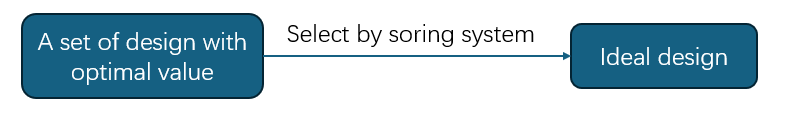
\includegraphics[width=0.7\textwidth,height=\textheight]{images/methods/method1.png}

}

\caption{\label{fig-method1}Method been used}

\end{figure}%

These approach separates the optimization of ED and NB from the A-value,
while I try to merge these two process into one algorithm. I use
pairwise permutation among treatments to change treatment design during
iterations. And to avoid design with bad ED and NB, I am using some
criteria to filter the permutation, only maintain or better properties
are accepted. In this way, a row-column design that satisfies multiple
optimization requirements is achieved.

\begin{figure}[H]

{\centering 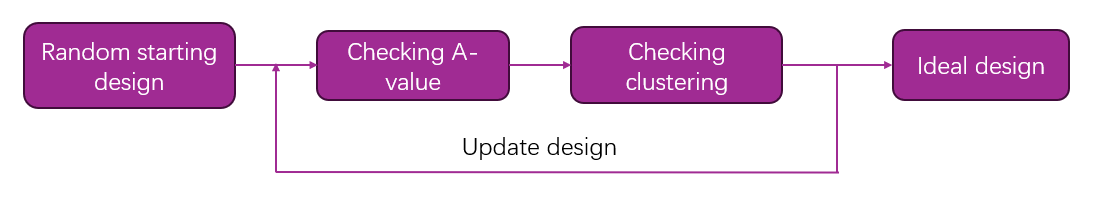
\includegraphics[width=0.7\textwidth,height=\textheight]{images/methods/method2.png}

}

\caption{Attempting method}

\end{figure}%

Basing on optimal design search methods share a common set of features
in exploring the design space given in \citet{butler2013optimal}, my
searching method contains following part:

\begin{enumerate}
\def\labelenumi{\arabic{enumi}.}
\item
  A calculation method for an optimal criterion for a given design
  matrix \(\boldsymbol{X}\)
\item
  An interchange policy to switch the design with in search space
  \(\Omega\)
\item
  An acceptance policy for a new design.
\item
  A stopping rule to terminate the search.
\end{enumerate}

The criterion calculation part has already been discussed earlier. We
will now introduce interchange policy of switching the design.

\subsection{Permutations and
filtering}\label{permutations-and-filtering}

We use permutations of the treatments to update the design matrix for
treatment. We randomly select two different treatments and swap them
within the design matrix during the permutation process, without making
drastic changes.

Let \(\boldsymbol{X}\) be the current design matrix for treatments,
where each row corresponds to an experimental unit, and each column
represents a treatment. Suppose we randomly select two different
treatments, \(t_i\) and \(t_j\) located in \(i\)th row and \(j\)th row
respectively. \(\boldsymbol{X}_{new}\) can be written as \[
\boldsymbol{X}_{new} = \boldsymbol{P}_{ij}\boldsymbol{X}
\] with permutation matrix defined as \[
 \boldsymbol{P}_{i j}=\left[
 \begin{array}{cccccccc}
 1 & 0 & \cdots & 0 & \cdots & 0 & \cdots & 0 \\ 
 0 & 1 & \cdots & 0 & \cdots &0 & \cdots & 0 \\ 
 \vdots & \vdots & \ddots & \vdots & & \vdots & \cdots & \vdots \\ 
 0 & 0 & \cdots & 0 & \cdots & 1 & \cdots & 0 \\
 \vdots & \vdots & & \vdots & \ddots & \vdots & & \vdots\\
 0 & 0 & \cdots & 1 & \cdots & 0 & \cdots & 0 \\ 
 \vdots & \vdots & \cdots & \vdots & & \vdots & \ddots & \vdots \\ 
 0 & 0 & \cdots & 0 & \cdots & 0 & \cdots & 1
 \end{array}\right] 
\] It is a identity matrix with \(i\)th row and \(j\)th row swapped.

When performing permutations on the design matrix, I apply checks based
on the metrics of evenness of distribution (ED) and neighbour balance
(NB). The goal is to ensure that only the permutations which improve or
at least maintain desirable values for ED and NB are accepted, while
others are filtered out.

A random permutation of treatments is generated by swapping two
different treatments in the design matrix, as described earlier using a
permutation matrix. Once the new design matrix \(\boldsymbol{X}_{new}\)
with corresponding design \(\mathcal{D}_{new}\) is created, the next
step is to evaluate the quality of the permutation by calculating the ED
and NB values for the new configuration. As afore-mentioned, we have NB
and ED criteria for \(\boldsymbol{X}_{new}\), that is \(C_{NB}'\),
\(MRS(\mathcal{D}_{new})\) and \(MCS(\mathcal{D}_{new})\). Comparing the
newly generated design matrix (offspring) with the original design
matrix (parent), We accept the new permutation, if the ED and NB values
improves or maintains them without significantly worse. In practice, we
often set a tolerance for the ED and NB values. We generally allow ED
and NB to become slightly worse, as it's not necessary for them to
strictly improve or remain unchanged in every iteration. Our goal is to
achieve a balance between ED, NB, and the A-value. For instance, ED
might increase slightly while NB decreases a little, as long as the
overall balance between the three objectives is maintained. This
approach has the added benefit of lowering the acceptance threshold for
permutations, which speeds up the algorithm during the random selection
process. For instance, we set tolerance for ED and NB as \(T_{ED}\) and
\(T_{NB}\), which are none negative numbers. Current design matrix
\(\boldsymbol{X}\) corresponding design \(\mathcal{D}\) has ED and NB
value\(C_{NB}\), \(MRS(\mathcal{D})\) and \(MCS(\mathcal{D})\). New
design matrix \(\boldsymbol{X}_{new}\) mentioned above is accepted when
\begin{equation}\phantomsection\label{eq-accp}{\begin{aligned}
&(C_{NB}'\leq C_{NB}+T_{NB}) \\
\land & (MRS(\mathcal{D}_{new})\geq MRS(\mathcal{D})-T_{ED})\\
\land & (MCS(\mathcal{D}_{new})\geq MCS(\mathcal{D})-T_{ED})
\end{aligned}}\end{equation} is true.

\subsection{Random search}\label{random-search}

The random search algorithm begins with a randomly selected design
matrix. To ensure that the search is efficient and avoids getting
trapped in local optima, we introduce the concept of step length. This
parameter determines how many permutations we consider in each
iteration. Given the computational constraints, especially when the
number of treatments or rows and columns increases, it is impractical to
check all possible permutations of a design and evaluate each for
acceptance. However, we aim to explore as many permutations as possible
to avoid falling into local optima.

At each iteration, we randomly generate a set of permutations. For each
generated permutation, we apply the filtering step check by
Equation~\ref{eq-accp}. If the permutation is not accepted, we randomly
select another one and repeat the process. This continues until we have
successfully selected a number of permutations equal to the step length.

We denote step length as \(s\). tolerance for ED and NB as \(t_{ED}\)
and \(t_{NB}\). For a design matrix \(\boldsymbol{X}\), its ED criteria
- minimum row span and minimum column span is, \(mrs({\boldsymbol{X}})\)
and \(mcs({\boldsymbol{X}})\), and NB criteria is denote as
\(C_{NB}({\boldsymbol{X}})\).

\begin{enumerate}
\def\labelenumi{\arabic{enumi}.}
\tightlist
\item
  \textbf{Input}: Original design matrix \(\boldsymbol{X}\), step length
  \(s\), tolerance for ED and NB as \(t_{ED}\) and \(t_{NB}\).
\item
  \textbf{Initialize}: \(k = 1\), ED and NB value for \(\boldsymbol{X}\)
  as \(mrs({\boldsymbol{X}})\), \(mcs({\boldsymbol{X}})\) and
  \(C_{NB}({\boldsymbol{X}})\).
\item
  While \(k < s\):

  \begin{itemize}
  \tightlist
  \item
    Generate a random permutation matrix \(\boldsymbol{P}\) by selecting
    two different treatments.
  \item
    Apply permutation: \(\boldsymbol{X_{new} = X P}\).
  \item
    Calculate new values of ED and NB, \(mrs({\boldsymbol{X}_{new}})\),
    \(mcs({\boldsymbol{X}_{new}})\) and
    \(C_{NB}({\boldsymbol{X}_{new}})\).
  \item
    If new values satisfy
    \(mrs({\boldsymbol{X}_{new}}) >= mrs({\boldsymbol{X}}) - t_{ED}\),
    \(mcs({\boldsymbol{X}_{new}}) >= mcs({\boldsymbol{X}}) - t_{ED}\)
    and
    \(C_{NB}({\boldsymbol{X}_{new}}) <= C_{NB}({\boldsymbol{X}}) + t_{NB}\),
    accept and remember this \(\boldsymbol{X}_{new}\).
  \item
    Increment \(k\).
  \item
    If \(k = s\), output all selected permutations.
  \end{itemize}
\item
  \textbf{Output}:A set of \(k\) permutations of original design matrix
  \(\boldsymbol{X}\)
\end{enumerate}

The Random Search algorithm starts with a randomly selected initial
design matrix \(\boldsymbol{X}_0\), and we aim to minimize the A-value
associated with the design. We set a maximum number of iterations \(M\)
and a step length \(s\).

The process for each iteration can be described as follows:

We denote a random design matrix \(\boldsymbol{X}_0\), and iteration
counter \(k\). Maximum number of iteration is \(M\). And denote the
A-value for a random design matrix \(\boldsymbol{X}\) is
\(A(\boldsymbol{X})\). Current design matrix during the iteration we
have is denoted as \(\boldsymbol{X}_c\)

\subsection{Simulated annealing}\label{simulated-annealing}

Simulated Annealing (SA) is a global optimization algorithm inspired by
the annealing process in metallurgy. At higher temperatures, the
algorithm allows the acceptance of worse solutions to escape local
optima; as the temperature decreases, it converges toward an optimal
solution.

\citet{butler2013optimal} state that the Boltzmann probability \[
P(E)\propto e^{[-E/kt]}
\] offer a pathway to measuring the accept possibility during the
algorithm, where \(E\) is the energy of the state,for a given
temperature \(t\). The constant \(k\) is Boltzmann's constant. The
energy \(E\) corresponds to the value of the objective function, in our
case is A-value. During the iterative process, suppose we have a design
(state) having A-value (energy) \(A_1\) at time \(t\), and we are
shifting our design into a new design with A-value \(A_2\), resulting in
an energy change \(A_{\bigtriangleup} = A_2 - A_1\). If
\(A_{\bigtriangleup}\) is negative, that is \(A_2 < A_1\), we always
accept new design since we have lower A-value. If \(A_{\bigtriangleup}\)
is positive, acceptance follows the Metropolis criterion: a random
number, \(\delta \in [0,1]\), is generated, and \(A_2\) is accepted if
\(\delta \leq exp(-A_{\bigtriangleup}/kt)\). So we have acceptance rate
\(P(A_2)\) for a new A-value \(A_2\).
\begin{equation}\phantomsection\label{eq-prob}{
P(A_2)=
\begin{cases}
1 & \text{if } A_2<A_1 \\
\exp(-A_{\bigtriangleup}/kt) & \text{if } A_2>A_1\\
\end{cases}
}\end{equation} The basic elements of SA given by
\citet{bertsimas1993simulated} is as followed

\begin{enumerate}
\def\labelenumi{\arabic{enumi}.}
\tightlist
\item
  A finite set \(S\).
\item
  A real-valued cost function \(J\) defined on \(S\). Let
  \(S^*\subset S\) be the set of global minima of the function \(J\),
  assumed to be a proper subset of \(S\).
\item
  For each \(i\in S\), a set \(S(i) \subset S - {i}\), called the set of
  neighbours of \(i\).
\item
  For every \(i\), a collection of positive coefficients \(q_{ij}\),
  \(j\in S(i)\), such that \(\sum_{j\in S(i)} q_{ij} = 1\). It is
  assumed that \(j\in S(i)\), if \(i \in S(j)\).
\item
  A nonincreasing function \(T:N\rightarrow (0, \infty)\), called the
  cooling schedule. Here \(N\) is the set of positive integers, and
  \(T(t)\) is called the temperature at time \(t\).
\item
  An initial ``state'' \(x(0)\in S\).
\end{enumerate}

We are applying these elements to a SA that fits our case. Our SA having
following elements.

\begin{enumerate}
\def\labelenumi{\arabic{enumi}.}
\tightlist
\item
  A finite searching space \(\{\boldsymbol{X}\}\) consisting all design
  matrix.
\item
  An A-value function \(A(\boldsymbol{X})\) defined on
  \(\{\boldsymbol{X}\}\) and it is real-valued. There is a set of
  \(\{\boldsymbol{X}^*\}\) that having optimal A-value and
  \(\{\boldsymbol{X}^*\}\in \{\boldsymbol{X}\}\)
\item
  For each design matrix \(\boldsymbol{X}\) in searching space, we
  consider all possible permutations filtered by Equation~\ref{eq-accp}
  are neighbours of \(\boldsymbol{X}\), which is a subset of searching
  space \(\{\boldsymbol{X}\}\).
\item
  All possible permutations have equal possibility to be chose, and the
  sum of the possibility it equal to \(1\).
\item
  A nonincreasing function \(T:N\rightarrow (0, \infty)\), \(T(t)\) is
  called the temperature at \(t\)-th iteration.
\item
  A random initial design \(\boldsymbol{X}_0\)
\end{enumerate}

Suppose we have a current design matrix \(\boldsymbol{X}_i\) and its
neighbours filtered by Equation~\ref{eq-accp} contains \(n_p\) numbers
of design. The next design is determined as follows:

A design matrix \(\boldsymbol{X}_j\) is randomly picked from the
neighbours of \(\boldsymbol{X}_i\). Suppose there is \(n_p\) design
matrices in the neighbours of \(\boldsymbol{X}_i\), then the probability
of selecting \(\boldsymbol{X}_j\) among all neighbours is
\(\frac{1}{n_p}\). This is actually the positive coefficients \(q_{ij}\)
afore-mentioned in basic elements of SA. We now denote
\(\boldsymbol{X}(t)\) to be the design matrix at \(t\)-th iteration.
Once \(\boldsymbol{X}_j\) is chosen, the next design matrix is
determined as follows: \[
P(\boldsymbol{X}(t+1)=\boldsymbol{X}_j|\boldsymbol{X}(t)=\boldsymbol{X}_i)
=\begin{cases}
1 & \text{if } A(\boldsymbol{X}_j)<A(\boldsymbol{X}_i) \\
\frac{1}{n_p}\exp(-(A(\boldsymbol{X}_j)-A(\boldsymbol{X}_i))/T(t) & \text{if } A(\boldsymbol{X}_j)>A(\boldsymbol{X}_i)\\
\end{cases}
\]

\subsubsection{Convergence analyze}\label{convergence-analyze}

In this section, We will discuss the convergence properties of the SA
algorithm. During iteration process, temperature cooling schedule plays
an important role in convergence. It determines whether the algorithm
will reach an optimal or near-optimal solution over time. Basing on work
in \citet{sasaki1988time}, \citet{bertsimas1993simulated} gives a
conclusion on convergence properties, with afore-mentioned basic
element. Define that state \(i\) communicates with \(S^*\) at height
\(h\) if there exists a path in \(S\) that starts at \(i\) and ends at
some element of \(S^*\) and the largest value of \(J\) along the path is
\(J(i)+h\). Denote \(d^*\) be the smallest number such that every
\(i \in S\) communicates with \(S^*\) at height \(d^*\).

The SA algorithm converges if and only if \[
\lim_{t\to 0} T(t)=0
\] and \begin{equation}\phantomsection\label{eq-covcon}{
\sum_{t=1}^{\infty} \exp[-\frac{d^*}{T(t)}]=\infty
}\end{equation}

To ensure the condition above, the mostly chose cooling schedule is
\begin{equation}\phantomsection\label{eq-logcol}{
T(t) = \frac{d}{\log t}
}\end{equation} Here \(d\) is some constant. It can be initial
temperature.

\begin{proof}
It is obvious that \(\lim_{t\to 0} T(t)=0\) in Equation~\ref{eq-logcol}

Bring Equation~\ref{eq-logcol} in to Equation~\ref{eq-covcon}, we have
\[
\sum_{t=1}^{\infty} \exp[-\frac{d^*\log (t)}{d}]=\sum_{t=1}^{\infty}t^{-\frac{d^*}{d}}
\] It is a harmonic series and it diverge when \(\frac{d^*}{d}<1\), that
is, \(d^*<d\). So SA of we have a large enough \(d\) (initial
temperature).
\end{proof}

Although logarithmic cooling theoretically guarantees convergence to the
global optimum, it is computationally demanding and has a very slow
convergence rate in practice, making it less feasible for large-scale
problems. To address these limitations, exponential cooling is
introduced as a more practical alternative. While it does not offer a
theoretical guarantee of reaching the global optimum, as noted by
\citet{kirkpatrick1983optimization}. Because of limited time and
computational resource, we will try to use exponential cooling in our as
given in \citet{aarts1989simulated} and well-practised It provides
near-optimal solutions within a reasonable time, making it highly
effective for large combinatorial optimization problems.
\begin{equation}\phantomsection\label{eq-expcol}{
T(t) = T_0 \exp(-\alpha*t)
}\end{equation} Here \(T_0\) is the initial temperature, and \(\alpha\)
is the cooling rate determine how fast the temperature drop.

\subsubsection{Algorithm}\label{algorithm}

For accept probability Equation~\ref{eq-prob}, we usually start with
\(0.8\) and keep dropping when iteration goes.This probability depends
on the magnitude of change in the objective function A-value. To
simplify the initialization, we often conduct a few preliminary
iterations to observe the range and rate of change in A-values, then use
these observations to determine an initial temperature. Several studies
have explored methods for autonomously selecting this initial
temperature.

\bookmarksetup{startatroot}

\chapter{Results}\label{sec-results}

\section{Simulation set-up}\label{simulation-set-up}

To begin the Results section, we'll look at the foundational set-up of
my simulation. In order to streamline the computation within limited
computational resources, I implemented a series of simplifications.

For \(\boldsymbol{G}\) matrix, I set it to be a diagonal matrix with
equal values along the diagonal. It implies that there is no correlation
between rows and columns, meaning that the effects for rows and columns
are considered independent. And the equal values along the diagonal
indicate that the variance of these row and column effects is the same.
In this simulation it is
\(\boldsymbol{G}_s = 10\boldsymbol{I}_{n_r+n_c}\)

For \(\boldsymbol{R}\) matrix, similarly, it is set as a diagonal matrix
with identical values along the diagonal. implying that the geographical
locations of different plots are independent of each other and variance
of residuals is uniform across plots. In this simulation it is
\(\boldsymbol{R}_s = 0.1\boldsymbol{I}_{n_r\times n_c}\)

To compare the differences between algorithms, we used the design
function from the R package blocksdesign to calculate the optimized
A-value \(A_{blocksdesign}\) basing on \citet{edmondson2020multi}, which
we then compared to the results from our iterative process.

For the consistency across all algorithms, we aimed to explore the
largest feasible range of row, column, and treatment combinations. We
set the maximum number of iterations \(M=2000\) for each algorithm. And
we add an early termination criterion: if the iterative algorithm's
A-value approaches \(A_{blocksdesign}\) within a specified tolerance
\(T_A\), the algorithm would stop iterating and output the A-value and
design matrix. In this simulation we set \(T_A=2\times 10^{-4}\)
Therefore we can evaluate the performance of different algorithms across
various combinations of row, column, and treatment numbers by comparing
the total computational time required, the actual iteration number
before reaching either \(M\) or an early termination based on
\(A_{blocksdesign}\), and the absolute difference between the
algorithm's and \(A_{blocksdesign}\).Basing on these evaluations, we can
identify how effectively each algorithm performs under different
complexity levels and determine the algorithm's efficiency and accuracy
across different cases.

In setting up random selection, the final parameter is the step length
\(s\). During runtime, the process of selecting permutations for
step-length iterations often accounts for a large portion of the total
functioning time.Additionally, this selection becomes especially
challenging when the row, column, and treatment numbers are low. In such
cases, while applying filtering criteria, it can be difficult to find a
sufficient number of unique permutations that meet the requirements, as
the design itself may not contain enough options. To ensure the
algorithm runs smoothly and completes within a reasonable time, we set
the step length to \(s=3\).

For the SA algorithm, we need to set the initial temperature \(T_0\).It
actually depends on the acceptance rate for higher A-values at the start
of the iteration process. As mentioned in the previous section, we
typically aim for an initial acceptance rate of around 0.8. That is we
hope \(\exp(-A_{\bigtriangleup}/T_0) \approx 0.8\). We often lack
precise information on \(A_{\bigtriangleup}\) before the algorithm, we
set the initial temperature based on an empirical estimate. We set
\(T_0=1\). Some adaptive algorithms for setting the initial temperature
are often discussed in the literature.

To examine combinations of row, column, and treatment numbers, we tested
a wide range of configurations. Row number ranged from 5 to 25, and
column number varied from 5 to 16. For each row and column combination,
we tested treatment numbers of 10, 20, 50, 80, and 100. To ensure that
the blocksdesign functions operated correctly and to maintain general
applicability, we ship a combination, if the product of rows and columns
was less than twice the treatment number.It ensures that each treatment
could have at least two replication. For each combination of row, column
and treatment number, we conduct three replication for more accurate
observation.

For the cases when treatment number cannot evenly divide the product of
rows and columns, suppose \(n_{plot}=n_r\times n_c\) and treatment
number is \(n_{\tau}\), we set base replication number as
\(\lfloor \frac{n_{plot}}{n_{\tau}} \rfloor\), and randomly pick
\(n_{plot}\quad mod\quad n_{\tau}\) treatments assign
\(\lfloor \frac{n_{plot}}{n_{\tau}} \rfloor+1\) replication to these
treatments. This approach ensures that the number of each treatment is
as close as possible to one another.

\section{Result analyze}\label{result-analyze}

\subsection{General behviour of
algorithms}\label{general-behviour-of-algorithms}

Now we observe the overall behaviour of the algorithm, to examine the
change of A-value during the process. We here use example with
\(n_c=n_r=15\) and \(n_\tau=50\). we now use blocksdesign functions to
generate a optimal design \(\mathcal{D}_{op}\) with A-value
\(A_{op} = 0.5027\) under set-up, NB criteria
\(C_{NB}(\mathcal{D}_{op})=3\) and ED criteria
\(MRS(\mathcal{D}_{op})=MCS(\mathcal{D}_{op})=5\). See detailed
assignment as follow

\begin{figure}[H]

{\centering 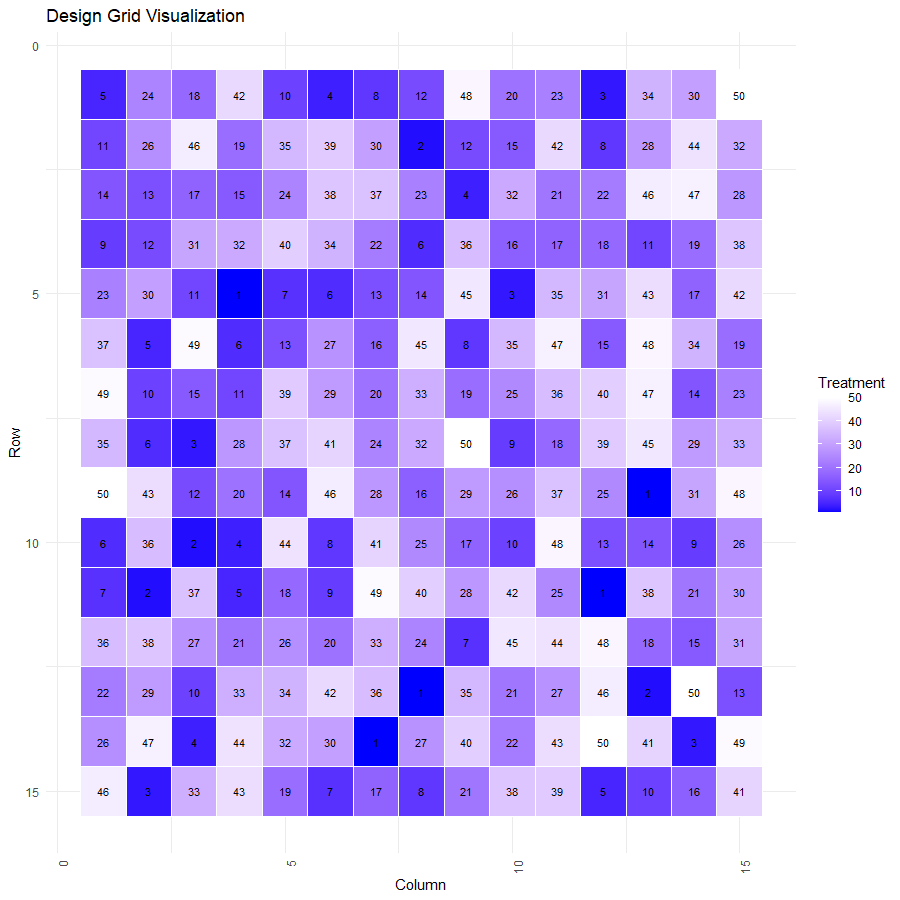
\includegraphics[width=0.7\textwidth,height=\textheight]{images/Rplots/block-design-visualization.png}

}

\caption{blocksdesign out put}

\end{figure}%

\subsubsection{Random selection}\label{random-selection}

We now look at how random selection behave during the process. The
iteration stops at \(549\)-th step with output A-value
\(A_{rs}=0.050478\) and NB criteria \(C_{NB}(\mathcal{D}_{rs})=4\) and
ED criteria \(MRS(\mathcal{D}_{rs})=5\) and \(MCS(\mathcal{D}_{rs})=7\).
The changes in the A-value over iterations and the specific design are
shown in the figure below.

\begin{figure}[H]

{\centering 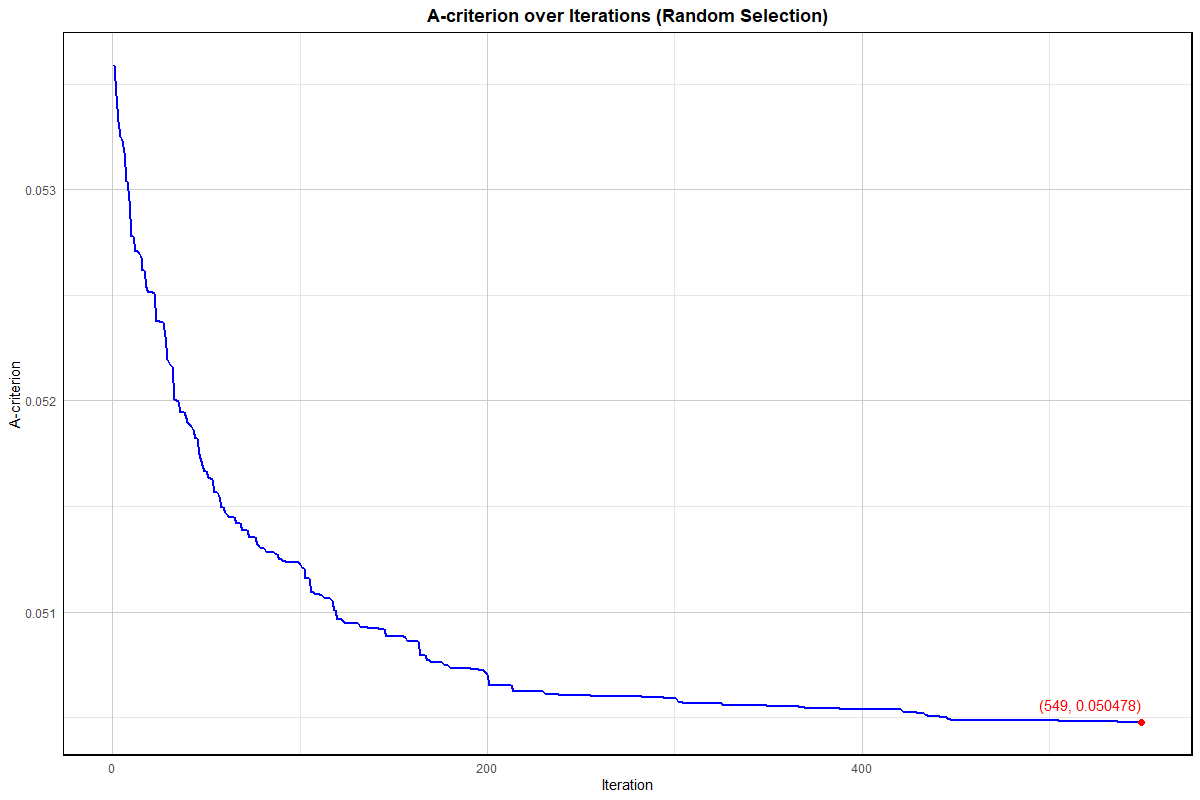
\includegraphics[width=0.7\textwidth,height=\textheight]{images/Rplots/random selection example.png}

}

\caption{A v.s. Iteration (Random search)}

\end{figure}%%
\begin{figure}[H]

{\centering 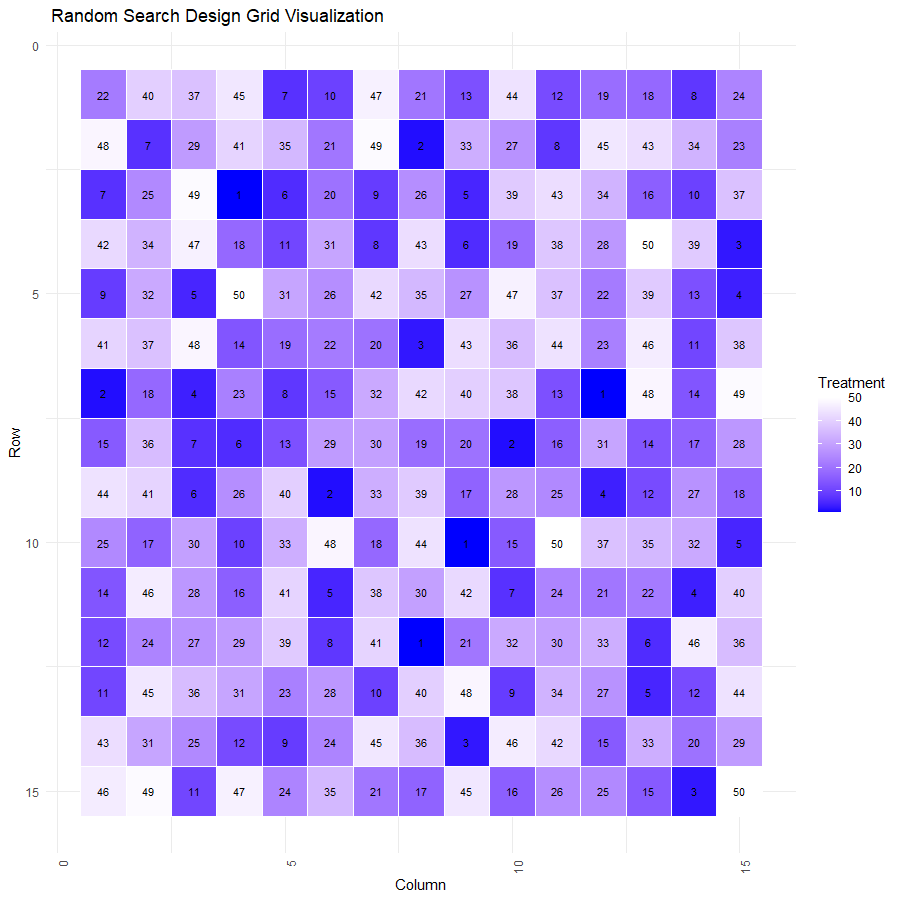
\includegraphics[width=0.7\textwidth,height=\textheight]{images/Rplots/Random search design visualization.png}

}

\caption{Random search out put design}

\end{figure}%

From the results, the A-value obtained by Random Search is relatively
close to that of the block design, though slightly larger, as is the NB
statistic. Recall that we would like A-value and \(C_{NB}\) to be as
small as possible, and for both \(MRC\) and \(MRC\), the larger the
better. Therefore, the Random Search outcome has a larger minimum column
span, meaning it preform better on evenness of distribution.

\subsubsection{SA with log cooling
schedule}\label{sa-with-log-cooling-schedule}

For SA using the log cooling schedule Equation~\ref{eq-logcol},Unlike
random selection, the algorithm accepts higher A-values with a certain
probability, causing fluctuations in A-values throughout the iterations,
resulting in rises and falls rather than a steady decline. Details can
be seen in the figure below.

\begin{figure}[H]

{\centering 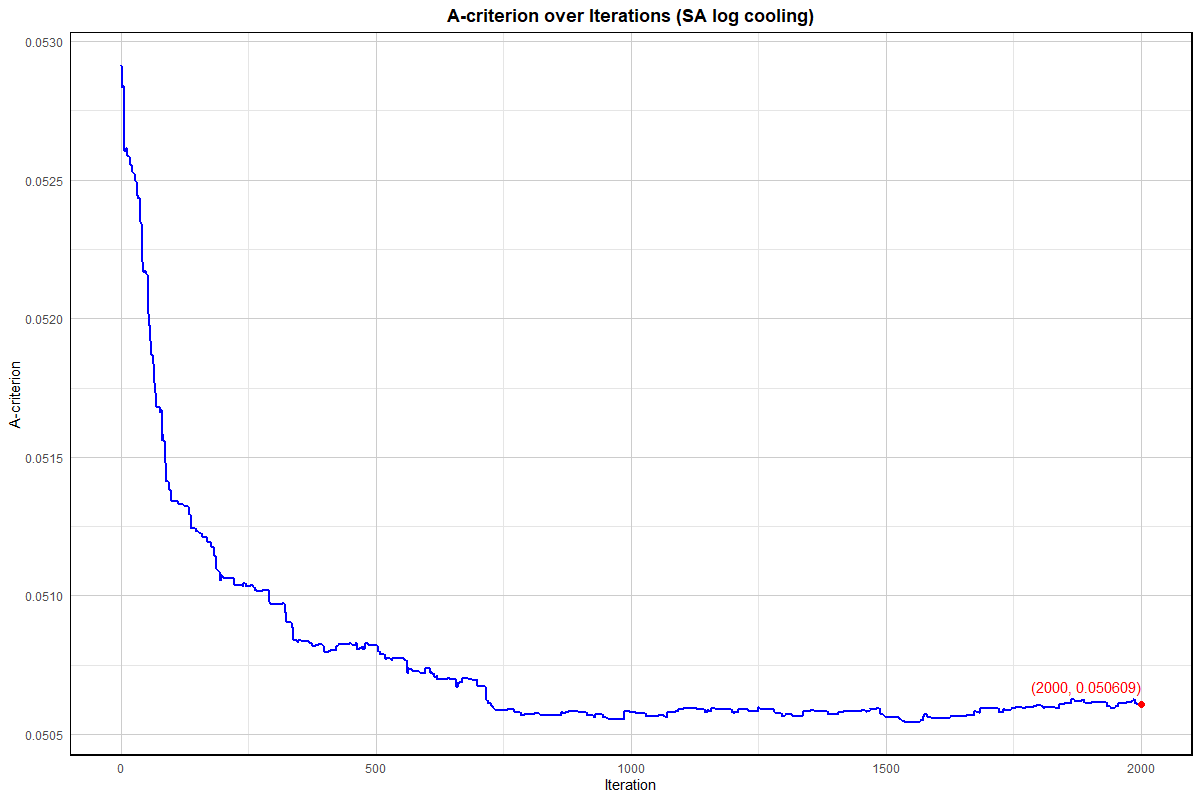
\includegraphics[width=0.7\textwidth,height=\textheight]{images/Rplots/SA_SLOW example.png}

}

\caption{A v.s. Iteration (SA with log cooling schedule)}

\end{figure}%%
\begin{figure}[H]

{\centering 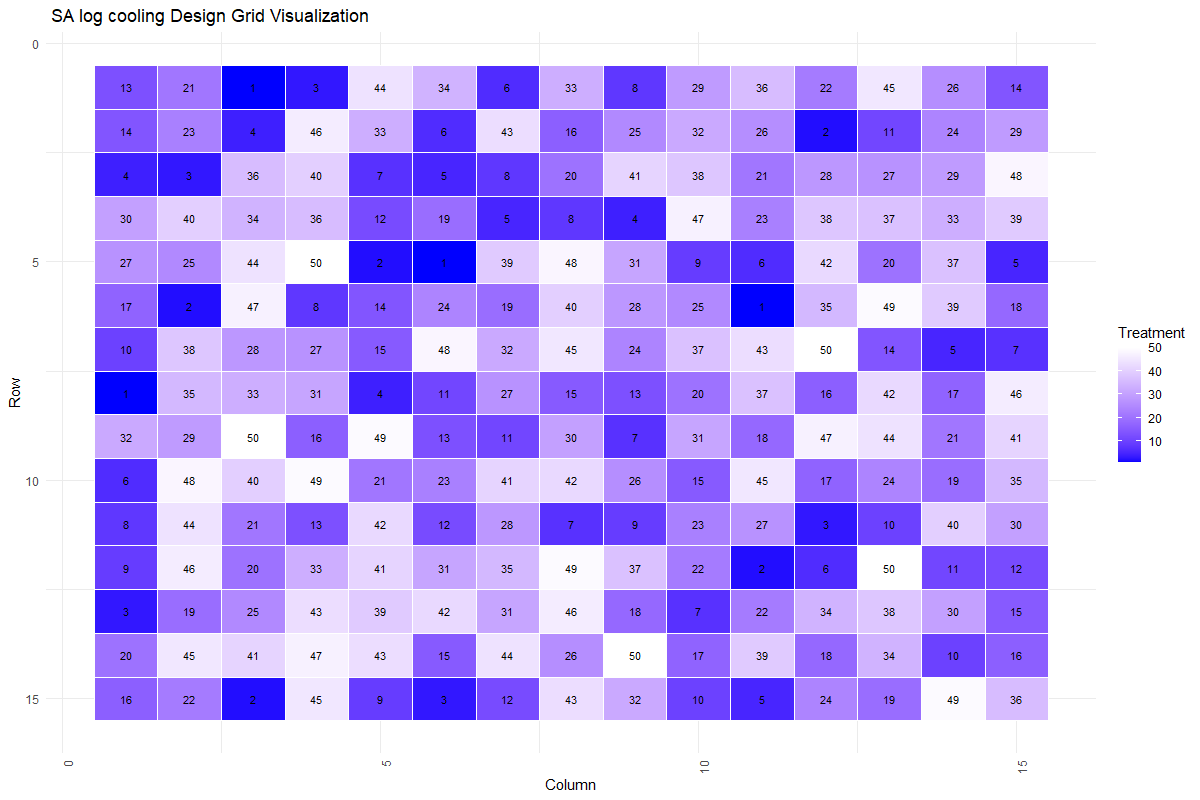
\includegraphics[width=0.7\textwidth,height=\textheight]{images/Rplots/SA_SLOW visualization.png}

}

\caption{SA with log cooling schedule out put design}

\end{figure}%

As it indicate in the plot, the process went through all iterations,
reaching maximum iteration number \(M\). At the 2000th iteration, the
A-value is \(A_{SAlog}=0.050609\) with NB criteria
\(C_{SAlog}(\mathcal{D}_{rs})=5\) and ED criteria
\(MRS(\mathcal{D}_{SAlog})=7\) and \(MCS(\mathcal{D}_{SAlog})=6\).

Compared to random selection, the optimization of the A-value in SA is
less effective, since the limitation of a maximum iteration number
\(M\).Similar to the NB statistic, where SA shows a less optimal outcome
than the block design. However, the two ED statistics given by SA are
significantly improved compared to those provided by the blockdesign
function and random selection. Because of the slower decrease in
acceptance rates for higher A-values with log cooling schedule, we
observe that the algorithm occasionally continues to accept larger
A-values even in the latter stages.

\subsubsection{SA with exp cooling
schedule}\label{sa-with-exp-cooling-schedule}

This is also SA but with an exponential cooling schedule
Equation~\ref{eq-expcol}. Although exponential cooling schedule does not
theoretically guarantee SA convergence to the global optimum, it can
produce a relatively near-optimal solution within finite computational
resources and time constraints. Because of the rapid temperature
decrease in exponential cooling, the algorithm initially shows
fluctuations in A-values at the beginning of the iterations. However, as
the number of iterations increases, the acceptance rate for larger
A-values declines quickly, and algorithm tend to avoid accepting higher
A-values.Details are shown in the figure below

\begin{figure}[H]

{\centering 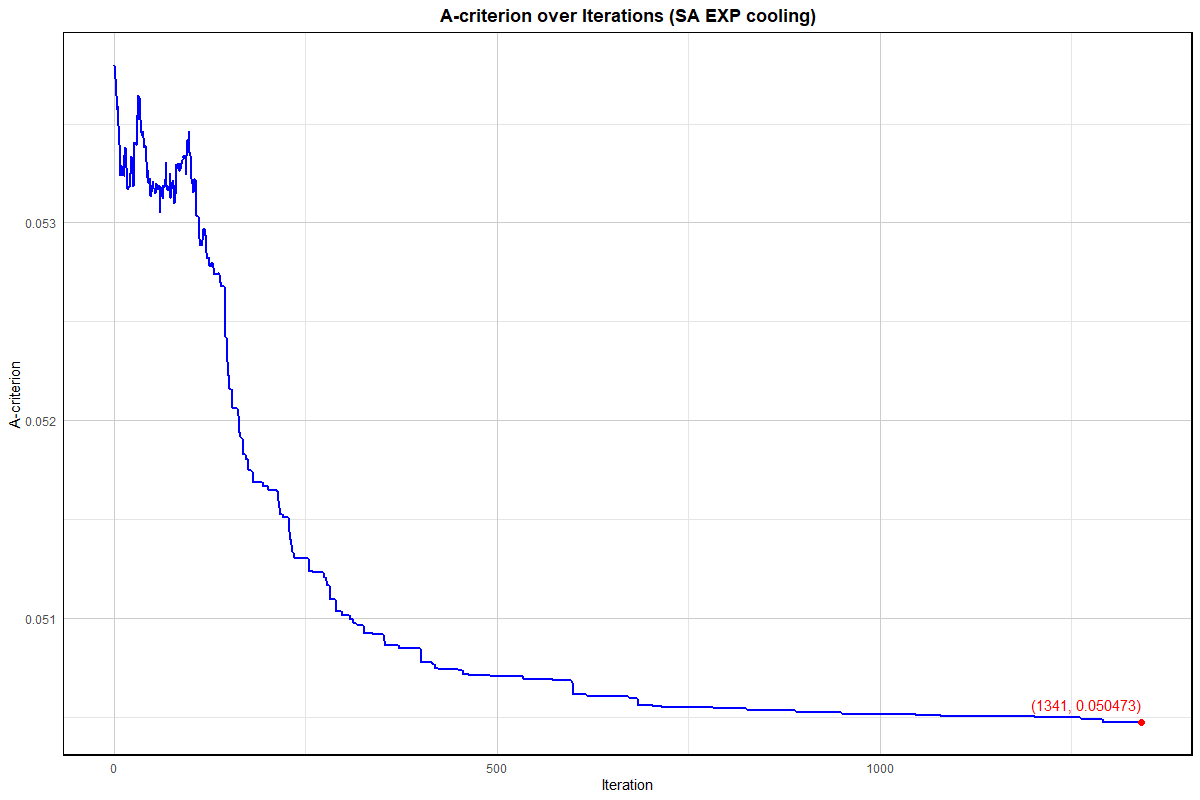
\includegraphics[width=0.7\textwidth,height=\textheight]{images/Rplots/SA_F example.png}

}

\caption{A v.s. Iteration (SA with exp cooling schedule)}

\end{figure}%%
\begin{figure}[H]

{\centering 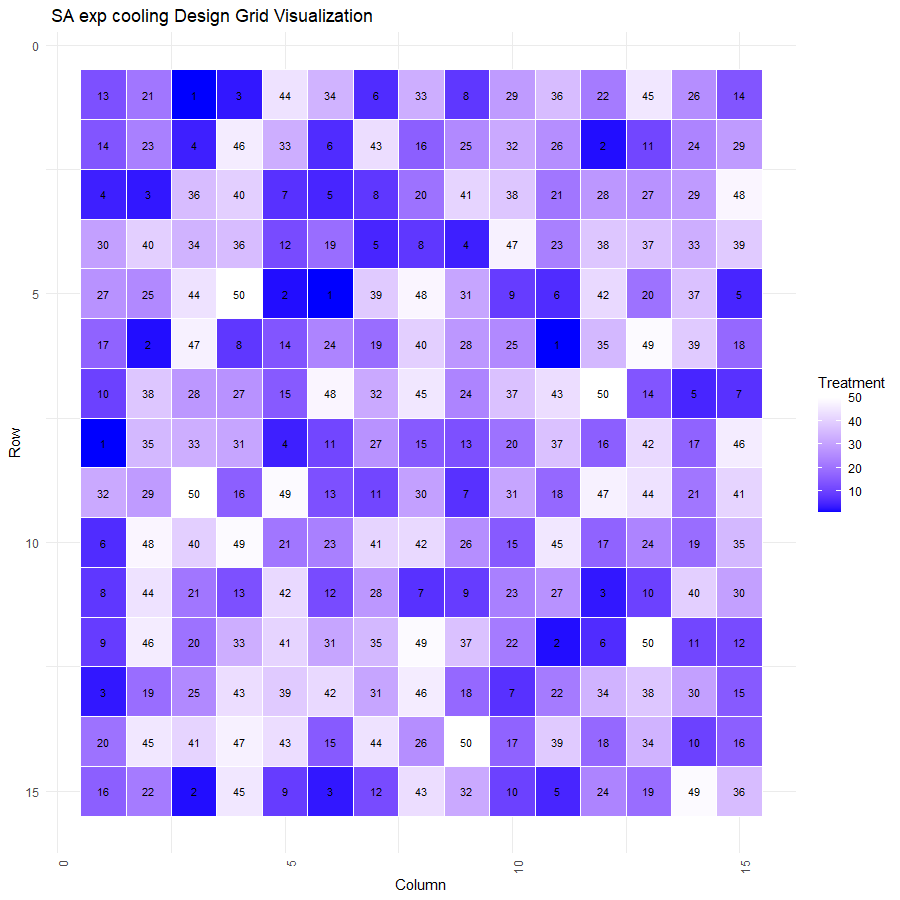
\includegraphics[width=0.7\textwidth,height=\textheight]{images/Rplots/SA_F visualization.png}

}

\caption{A v.s. Iteration (SA with exp cooling schedule)}

\end{figure}%

The iteration process stopped at the \(1341\)-st iteration because the
A-value had come sufficiently close to the blockdesign A-value. The
results show that the A-value achieved is \(A_{SAexp} = 0.050473\), with
an NB statistic \(C_{SAexp}(\mathcal{D}_{rs})=4\), and ED statistics
\(MRS(\mathcal{D}_{SAexp})=5\) and \(MCS(\mathcal{D}_{SAexp})=6\).

The exponential cooling schedule achieved similar A-values and NB
statistics to those of random selection. However, its performance on the
ED statistic was less effective compared to both random selection and
log cooling. The reason may be the early termination of iterations in
exponential cooling, which limited the exploration of the whole design
matrix space.

In contrast, random selection evaluates multiple permutations (equal to
the step length \(s\)) in each iteration, which allows it to consider a
broader range of potential solutions. Meanwhile, log cooling slows down
the convergence, allow it has sufficient iterations to explore the
solution space, although it selects only one neighbour at a time.

\subsection{Analysis by Algorithm}\label{analysis-by-algorithm}

Now we begin to explore the relationship between function runtime and
the number of rows, columns, and treatments. Generally, runtime is
proportional to the number of iterations. Here, we have set the maximum
number of iterations to 2000. If in the simulation most runs reach the
maximum number of iterations, then evaluating the relationship between
runtime and rows, columns, and treatment numbers will no longer be
meaningful.Therefore, before the analysis, we need to examine the
distribution of iteration numbers. If most of the simulations do not
reach the maximum number of iterations, we can use runtime as a measure
of computational efficiency.

For random selection, many simulations did not reach the maximum number
of iterations, which can be observed in the figure.

\begin{figure}[H]

{\centering 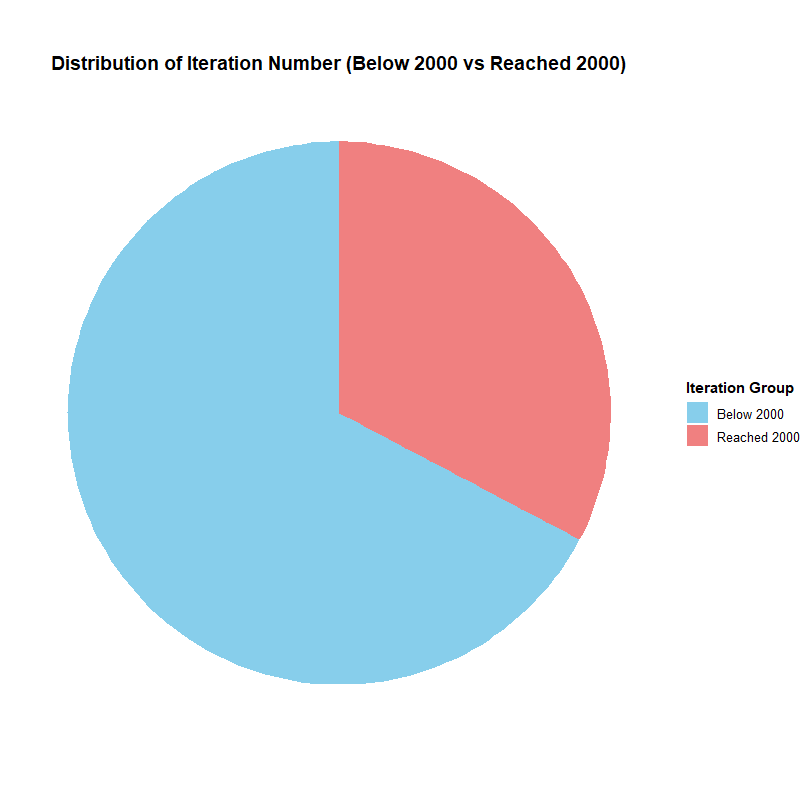
\includegraphics[width=0.7\textwidth,height=\textheight]{images/Rplots/RS_eva/RS-iternum-distribution.png}

}

\caption{\#rows v.s. runtime (random selection)}

\end{figure}%

So we present the relationship between runtime and the number of rows
under different treatment numbers, as shown in the figures below. As
mentioned earlier, we have three replications for each combination of
rows, columns, and treatment numbers. We calculate the average of the
three replications for each combination as the final result.

\begin{figure}[H]

{\centering 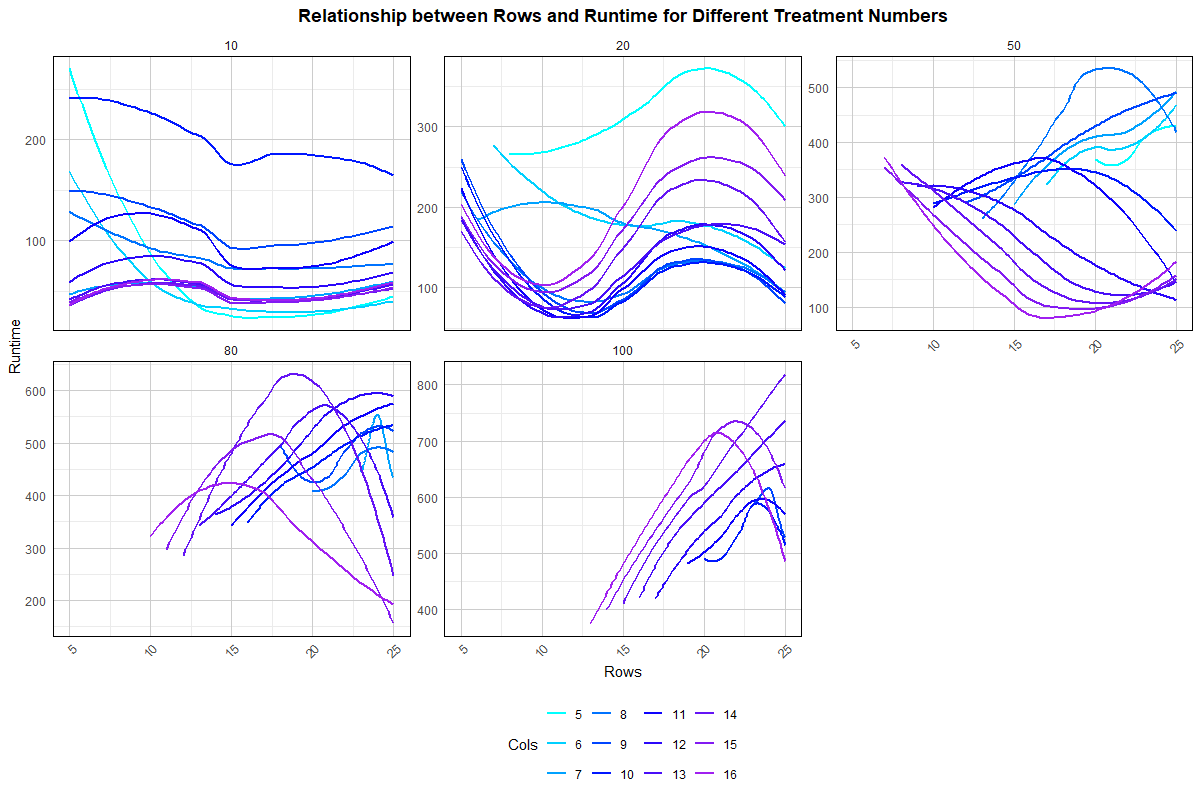
\includegraphics[width=0.7\textwidth,height=\textheight]{images/Rplots/RS_eva/RS-row-vs-runtime.png}

}

\caption{\#rows v.s. runtime (random selection)}

\end{figure}%

We can observe that, under different numbers of columns, the
relationship between rows and runtime tends to be similar. Here, we will
not discuss the origin or significance of this trend but instead focus
on the relation between variables and runtime. There is no clear
positive or negative relationship between the number of rows and
runtime. We see that as the number of rows increases, the runtime does
not consistently increase or decrease, which is related to the
randomness of random selection. During the iteration process, we might
be lucky enough to find a good design early and terminate the iteration,
or the A-value may gradually decrease over the iterations.

However, by observing the vertical axis of different subplots, we can
see that as the number of treatments increases, the range of runtime
fluctuations also increases. To demonstrate this, we present the
relationship between the number of treatments and runtime under
different rows and columns.

\begin{figure}[H]

{\centering 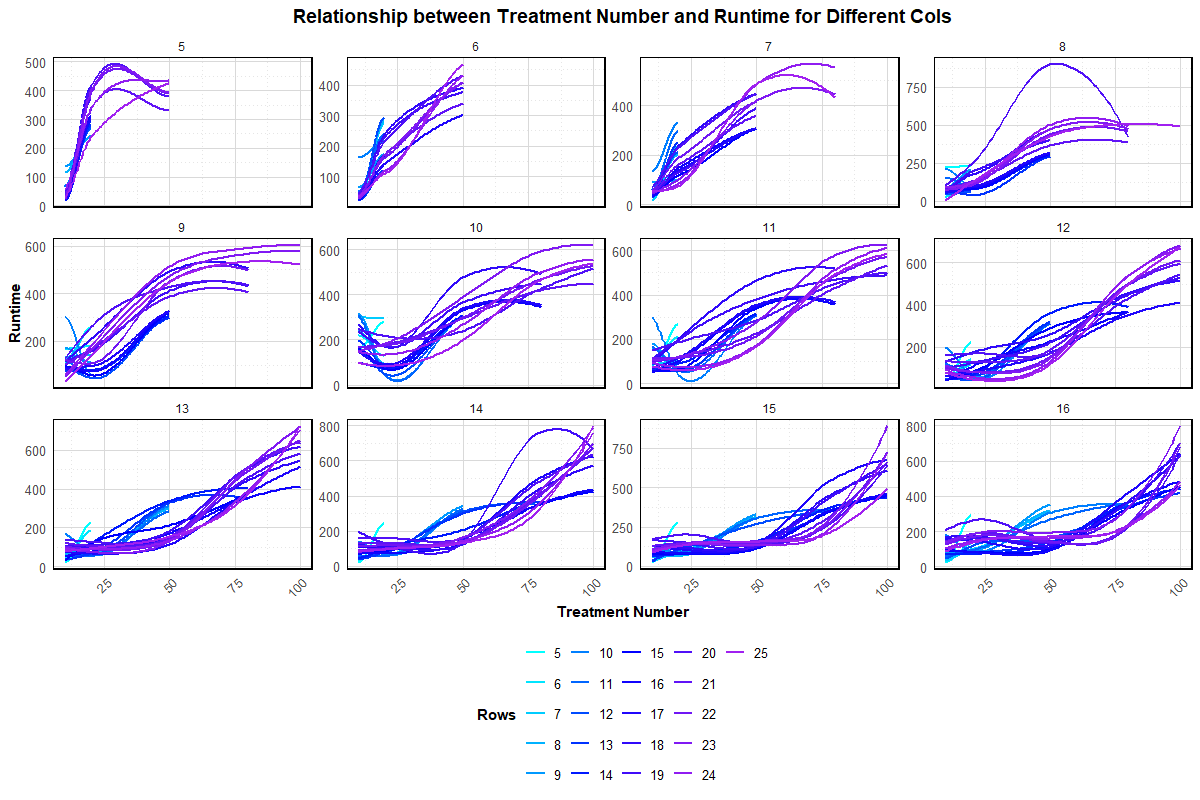
\includegraphics[width=0.7\textwidth,height=\textheight]{images/Rplots/RS_eva/RS-trt-vs-runtime.png}

}

\caption{\#treatment v.s. runtime (random selection)}

\end{figure}%

By observing the figure, we can see that as the number of treatments
increases, runtime shows a positive correlation, indicating that with
more treatments, random selection requires more time to find
permutations and make comparisons.

This approach leads us to consider the relationship between the number
of treatments and runtime. However, for SA with log cooling, due to the
slow convergence of log cooling and the limitation of a maximum number
of iterations, the algorithm often runs until the maximum number of
iterations is reached. This makes it difficult to observe the
relationship between the number of treatments and runtime, as runtime is
often related to the maximum number of iterations. See the image below
for details.

\begin{figure}[H]

{\centering 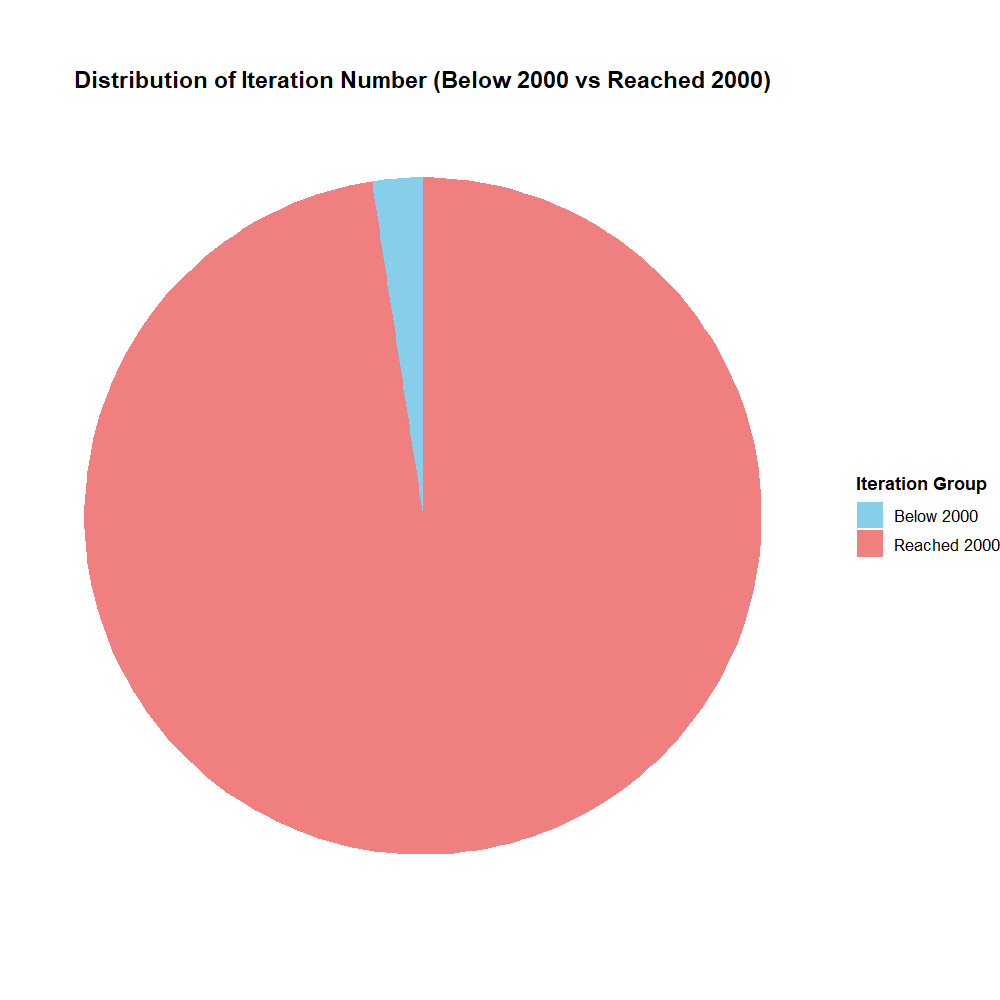
\includegraphics[width=0.7\textwidth,height=\textheight]{images/Rplots/SA-Slow-eva/SA-Slow-iternum-distribution.png}

}

\caption{Iteration number distribution (SA with log cooling schedule)}

\end{figure}%

In the figure, we can see that only when the number of rows and columns
is small, meaning the design space is limited, SA with log cooling can
terminate before reaching the maximum number of iterations. In most
other cases, the algorithm stops when it reaches the maximum number of
iterations. Therefore, we use the difference
\(d = (A_{SAlog}-A_{op})/A_{op}\) between the A-value obtained by SA
with log cooling at the maximum number of iterations and the A-value
calculated by the blockdesign function to evaluate the impact of the
number of rows, columns, and treatments on the efficiency of the
algorithm.

We first look at the influence of the number of rows on the distance.
Similar to the analysis method used for random selection, we provide the
following figure.

\begin{figure}[H]

{\centering 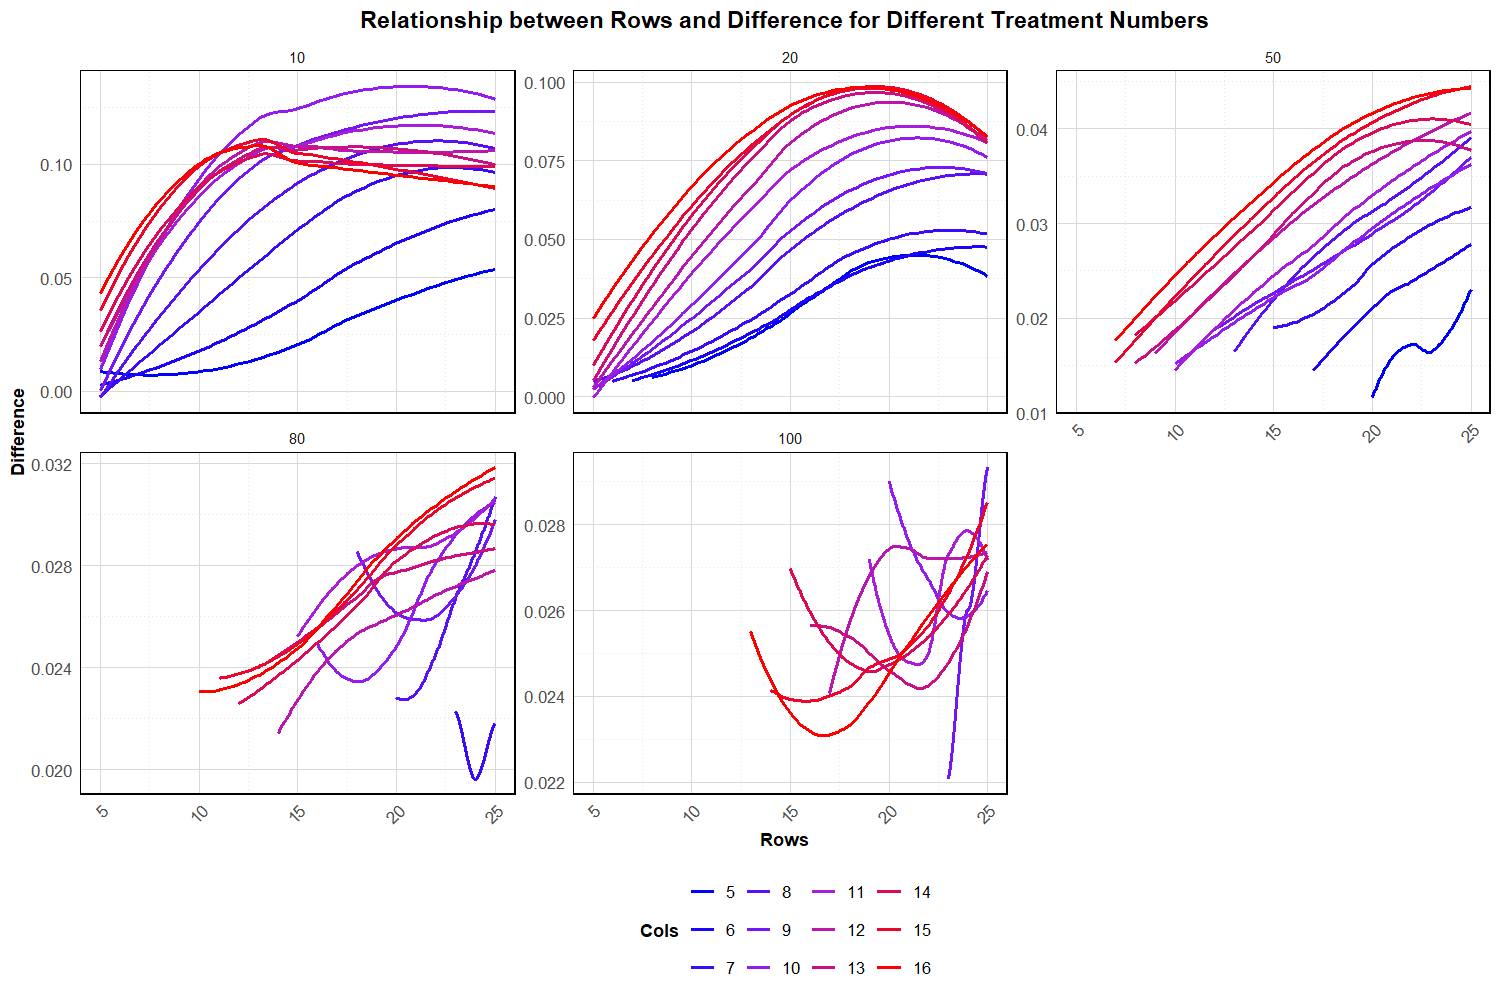
\includegraphics[width=0.7\textwidth,height=\textheight]{images/Rplots/SA-Slow-eva/SA-Slow-row-vs-diff.png}

}

\caption{\#rows v.s. difference (SA with exp cooling schedule)}

\end{figure}%

From the above figure, it is evident that the number of rows and columns
is positively correlated with the difference. The greater the number of
rows, the larger the difference. Similarly, the greater the number of
columns, the higher the lines (towards the red), indicating a larger
difference. Based on previous experience, we attempt to examine the
relationship between the number of treatments and distance, as shown in
the figure below.

\begin{figure}[H]

{\centering 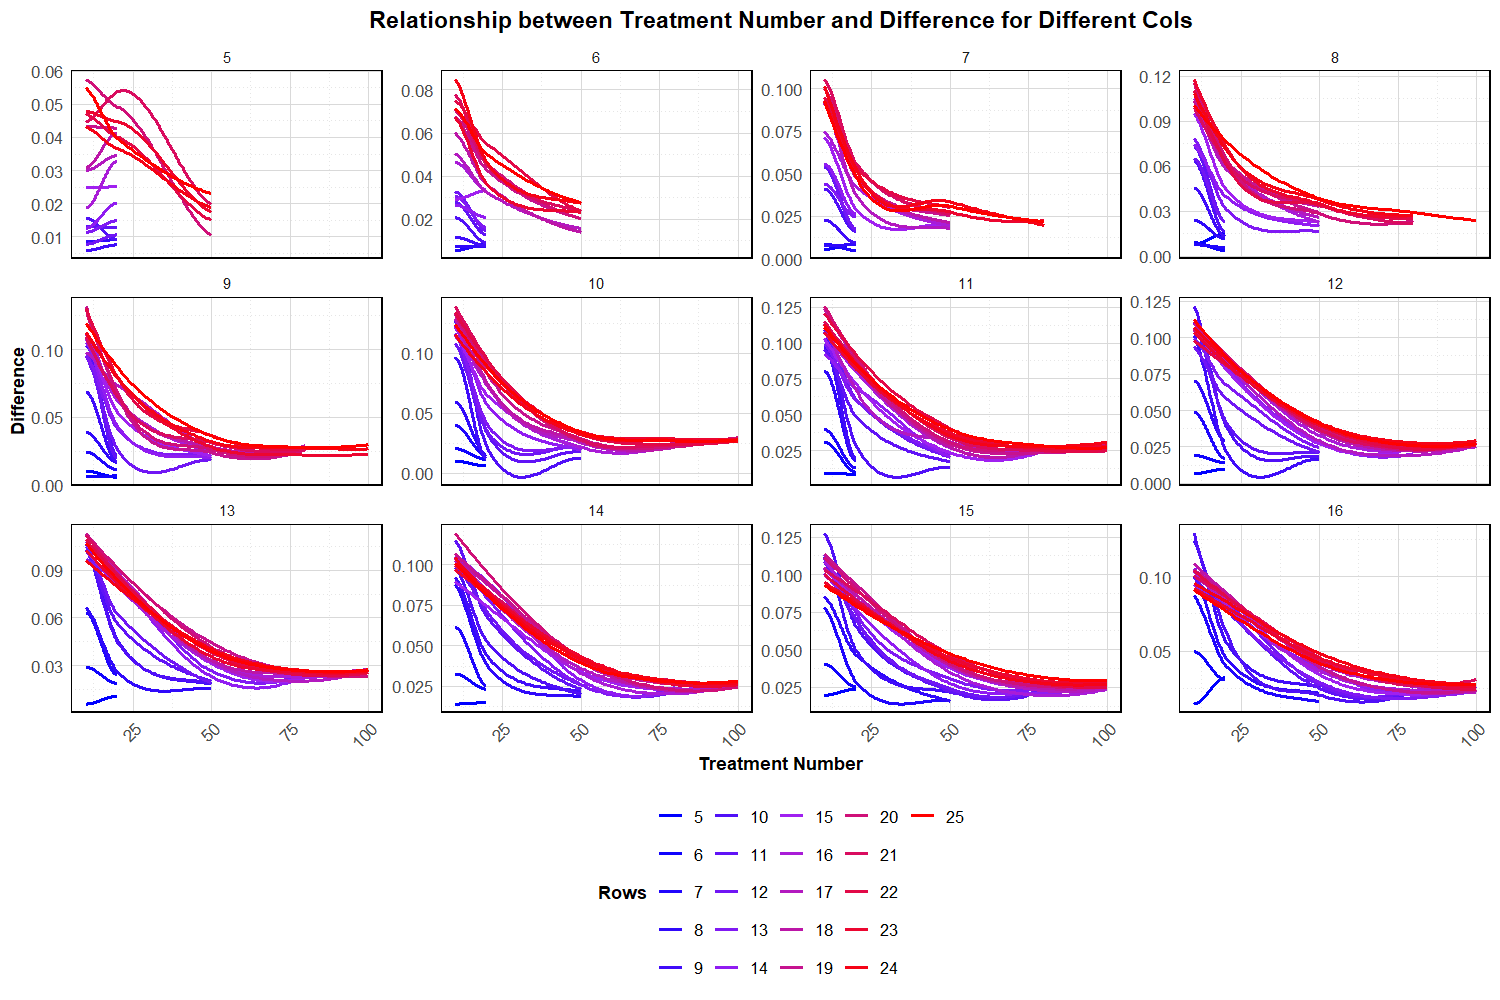
\includegraphics[width=0.7\textwidth,height=\textheight]{images/Rplots/SA-Slow-eva/SA-Slow-trt-vs-diff.png}

}

\caption{\#treatment v.s. difference (SA with exp cooling schedule)}

\end{figure}%

The results show that the treatment number is negatively correlated with
the difference. In other words, as the treatment number increases, the
resulting value (whether the iteration stops early or reaches the
maximum number of iterations) tends to be closer to the optimal value.
However, this does not necessarily mean that the absolute distance to
the optimal value decreases.

For SA with exponential cooling, we also examine the distribution of the
iteration numbers.

\begin{figure}[H]

{\centering 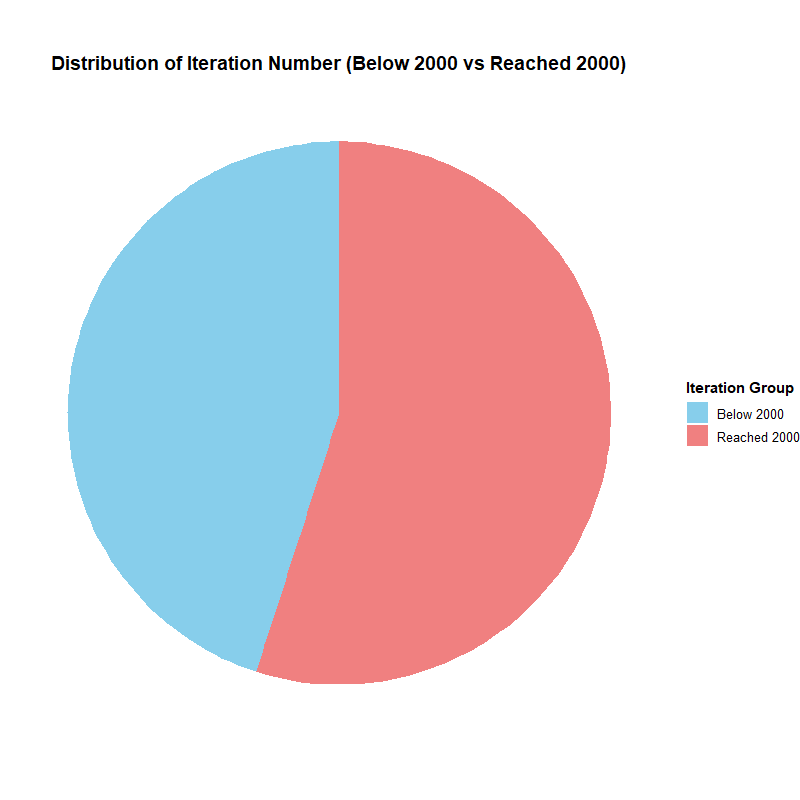
\includegraphics[width=0.7\textwidth,height=\textheight]{images/Rplots/SA-Fast-eva/SA-Fast-iternum-distribution.png}

}

\caption{\#rows v.s. runtime (random selection)}

\end{figure}%

It can be seen that most of the simulations did not reach the maximum
number of iterations, so we can use runtime to compare the effects of
rows, columns, and treatment numbers on the algorithm.

\begin{figure}[H]

{\centering 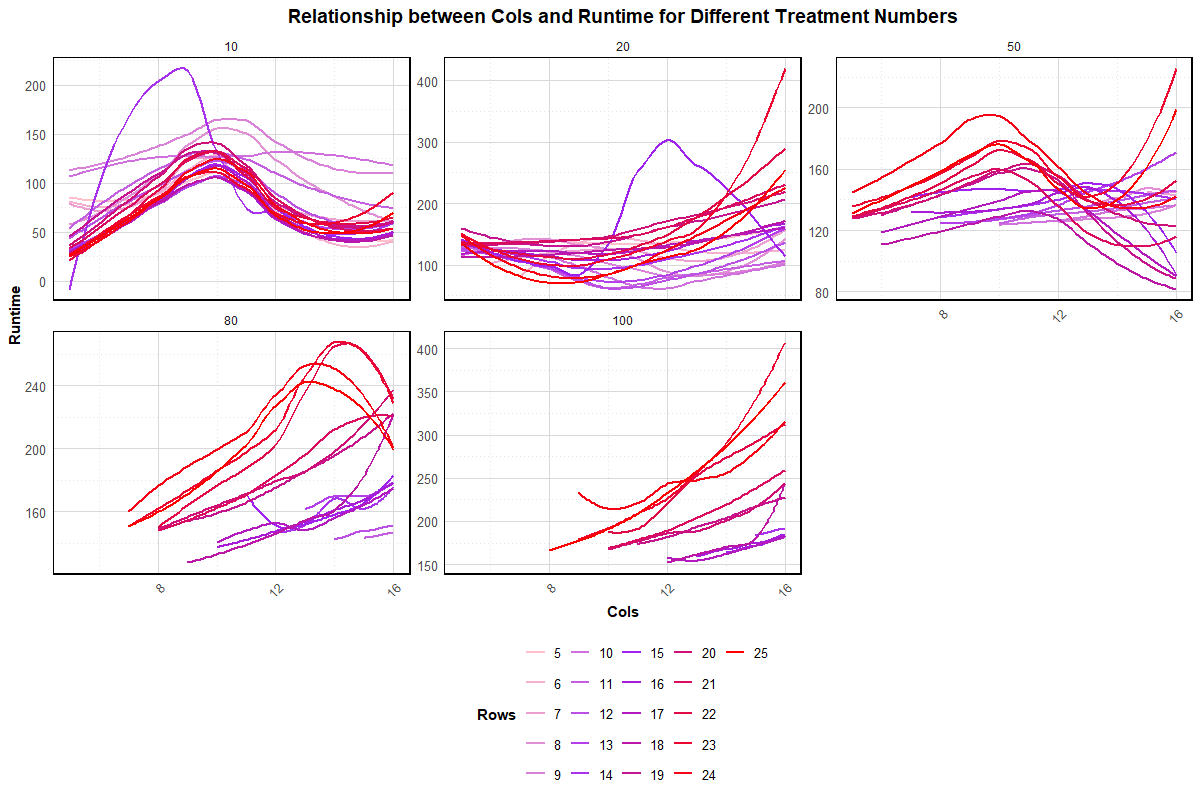
\includegraphics[width=0.7\textwidth,height=\textheight]{images/Rplots/SA-Fast-eva/SA-Fast-row-vs-runtime.png}

}

\caption{\#rows v.s. runtime (random selection)}

\end{figure}%

We can see that when the treatment number is small, the influence of
rows and columns on runtime is not significant. This could be because
the design space is smaller, and for randomness, the algorithm stops
after fewer iterations. As the treatment number increases, the impact of
rows and columns on runtime becomes apparent: the greater the number of
rows and columns, the longer the runtime.This effect can also be
observed when examining the influence of the treatment number on
runtime.

\begin{figure}[H]

{\centering 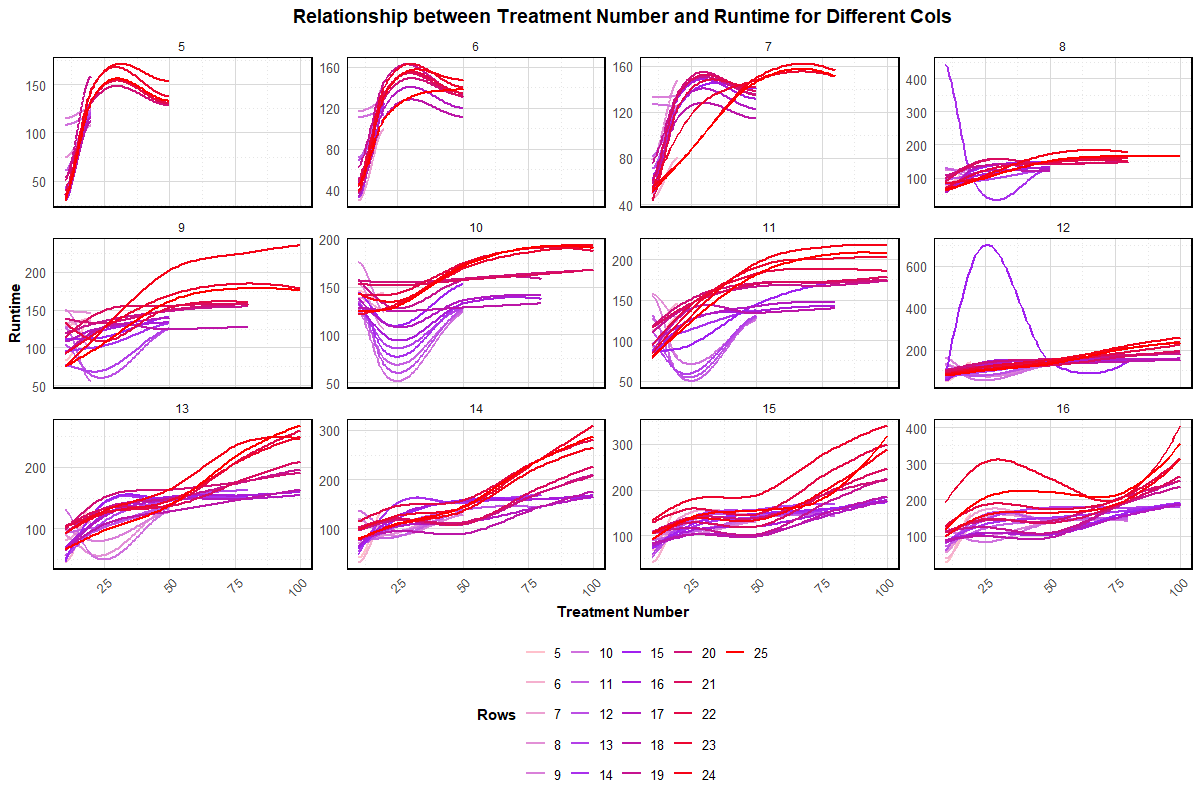
\includegraphics[width=0.7\textwidth,height=\textheight]{images/Rplots/SA-Fast-eva/SA-Fast-trt-vs-runtime.png}

}

\caption{\#rows v.s. runtime (random selection)}

\end{figure}%

Similarly, we can observe that as the treatment number increases, the
runtime also increases. Additionally, as the number of rows increases,
the vertical axis of the plot also grows, indicating their positive
correlation.

\subsection{Comparison Between
Algorithms}\label{comparison-between-algorithms}

Now we compare the effectiveness of different algorithms. To simplify
the process, we focus on observing the impact of the number of rows,
columns, and treatments on the average runtime and the average
difference under equivalent conditions. For example, when comparing the
effect of the number of rows on the difference for different algorithms,
we take the average of the difference for different column counts and
treatment numbers at the same row level to simplify the visualization
and makes the comparison more intuitive. Before making comparisons, it
is important to note that, for our computational resource limitations,
we have limited the maximum iteration number to 2000. Therefore, our
comparison cannot determine which algorithm is better. Therefore, it
aims to compare the performance of different algorithms under the same
computational constraints. Here, we compare the effects of row number,
column number, and treatment number on the difference and runtime across
different algorithms.

\subsubsection{Comparing with
difference}\label{comparing-with-difference}

Now, we use the difference to compare the computational efficiency of
different algorithms. We present the figures showing the influence of
row number, column number, and treatment number on the difference for
the three algorithms. Note that for random selection and SA with
exponential cooling, the method for calculating the difference is the
same as for SA with logarithmic cooling, which means it represents the
relative difference, that is \(d = (A_{op}-A_{result})/A_{op}\).

\begin{figure}[H]

{\centering 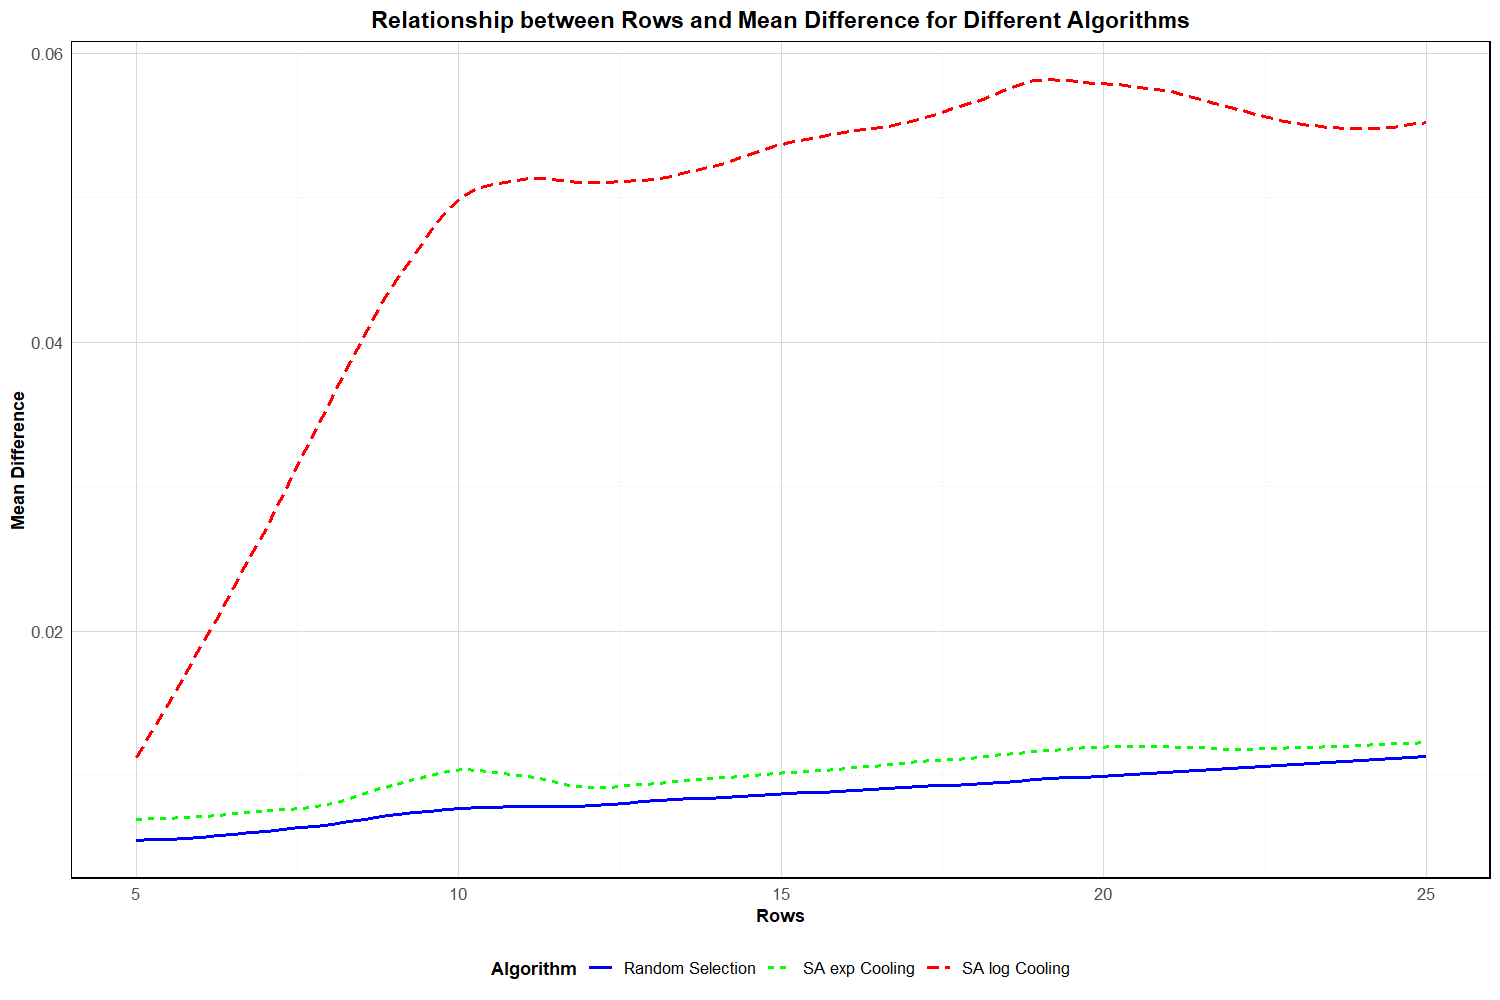
\includegraphics[width=0.7\textwidth,height=\textheight]{images/Rplots/means/r-vs-D.png}

}

\caption{\#rows v.s. difference)}

\end{figure}%%
\begin{figure}[H]

{\centering 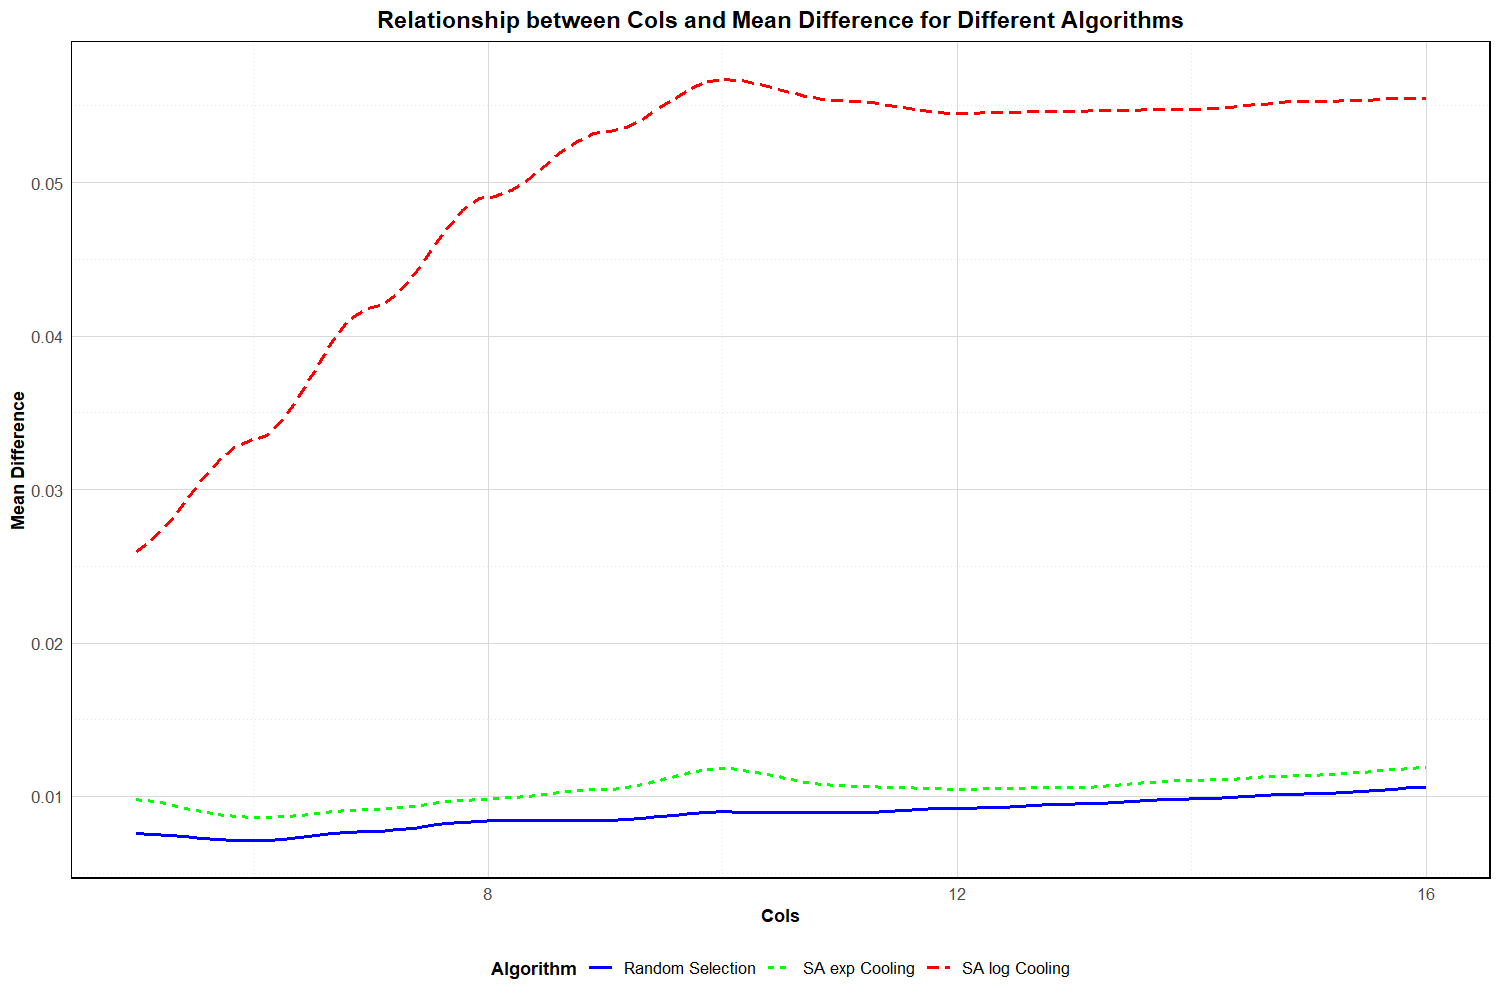
\includegraphics[width=0.7\textwidth,height=\textheight]{images/Rplots/means/c-vs-D.png}

}

\caption{\#rows v.s. difference)}

\end{figure}%%
\begin{figure}[H]

{\centering 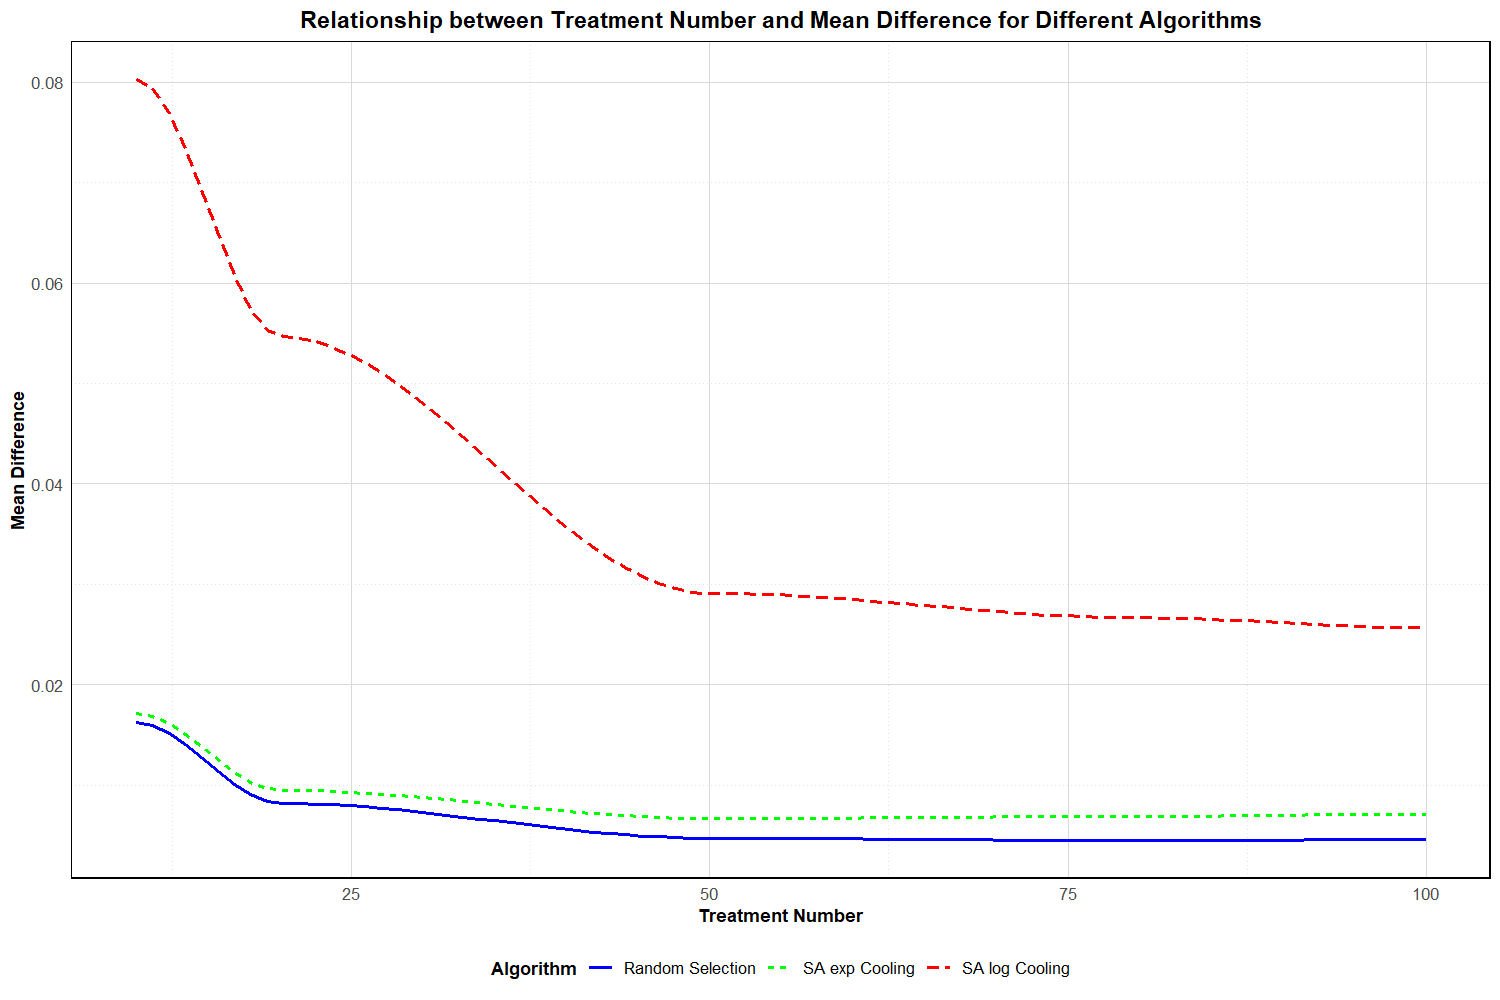
\includegraphics[width=0.7\textwidth,height=\textheight]{images/Rplots/means/trt-vs-D.png}

}

\caption{\#rows v.s. difference)}

\end{figure}%

Overall, it can be observed that for the difference, random selection
has the smallest value, SA with exponential cooling is slightly larger,
and SA with logarithmic cooling has the largest value. Moreover, SA with
logarithmic cooling is more influenced by the three variables.

In general, for all three algorithms, as the number of rows and columns
increases, the relative difference also increases. However, the
difference is negatively correlated with the treatment number. As
mentioned earlier, a smaller relative difference does not necessarily
mean that the absolute distance to the optimal value decreases. We can
use the figure below to support this point.

\begin{figure}[H]

{\centering 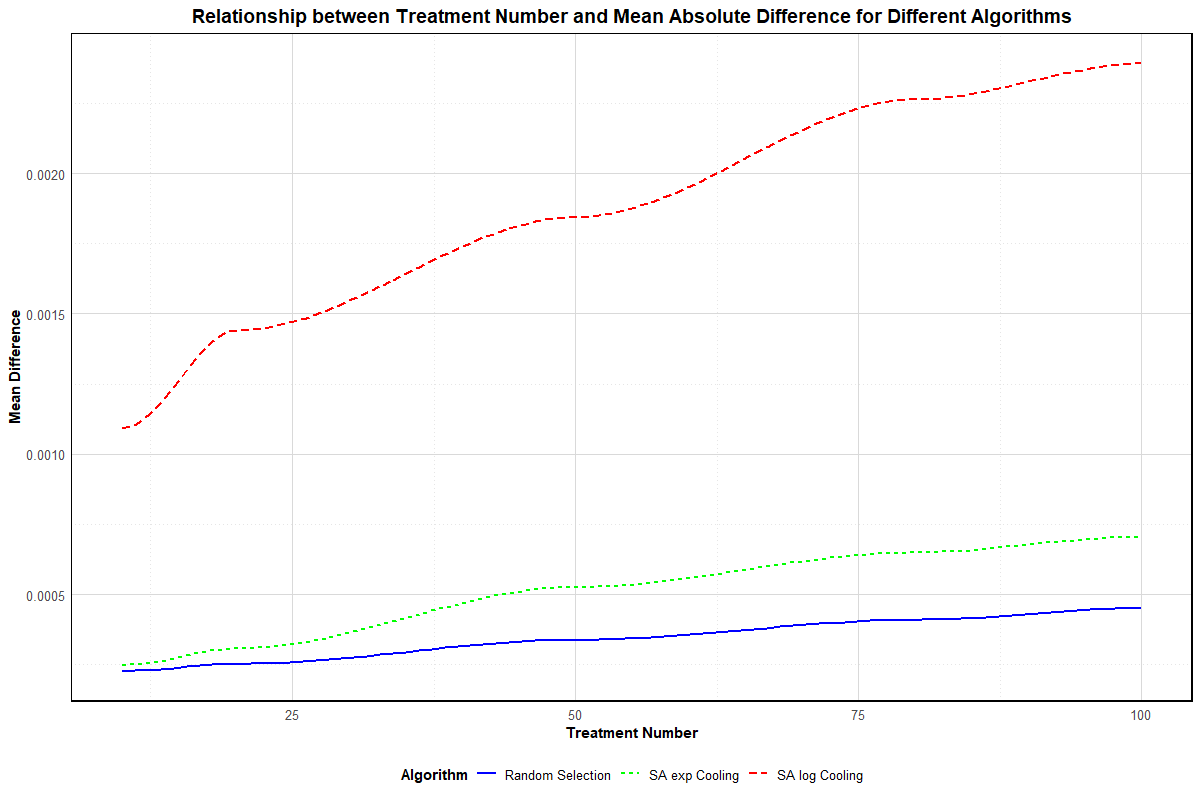
\includegraphics[width=0.7\textwidth,height=\textheight]{images/Rplots/means/trt-vs-ABS-D.png}

}

\caption{\#rows v.s. difference)}

\end{figure}%

It can be seen here that if we consider the absolute difference, it is
actually positively correlated with the treatment number.

\subsubsection{Comparing with runtime}\label{comparing-with-runtime}

Now, let's see what the comparison looks like from the perspective of
runtime. We present the following figure to illustrate this.

\begin{figure}[H]

{\centering 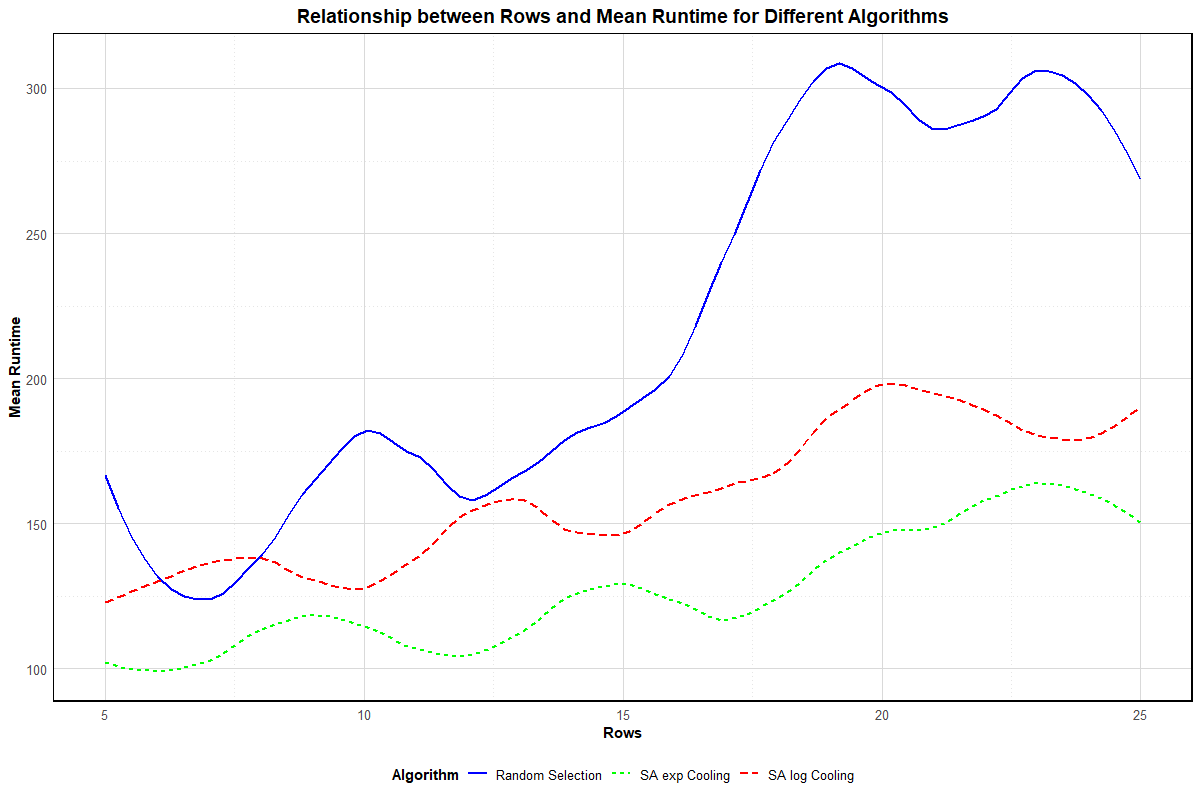
\includegraphics[width=0.7\textwidth,height=\textheight]{images/Rplots/means/r-vs-t.png}

}

\caption{\#rows v.s. difference)}

\end{figure}%%
\begin{figure}[H]

{\centering 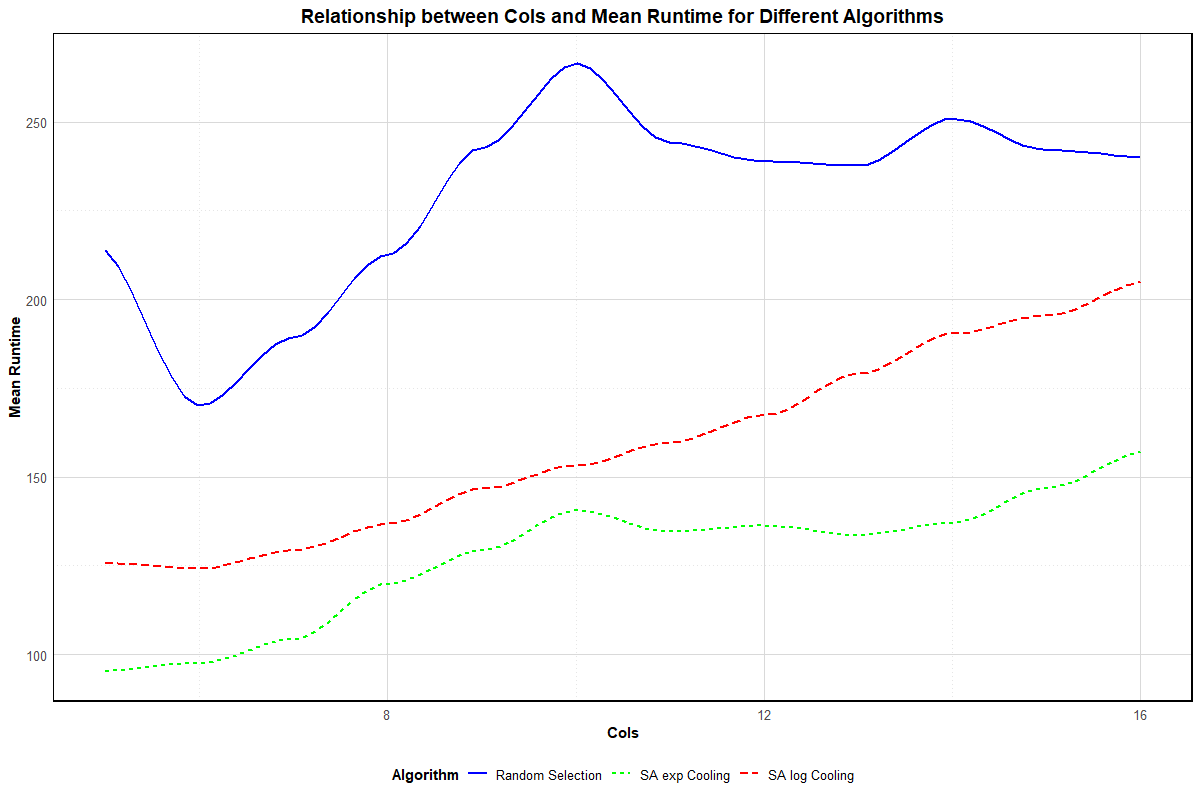
\includegraphics[width=0.7\textwidth,height=\textheight]{images/Rplots/means/c-vs-t.png}

}

\caption{\#rows v.s. difference)}

\end{figure}%%
\begin{figure}[H]

{\centering 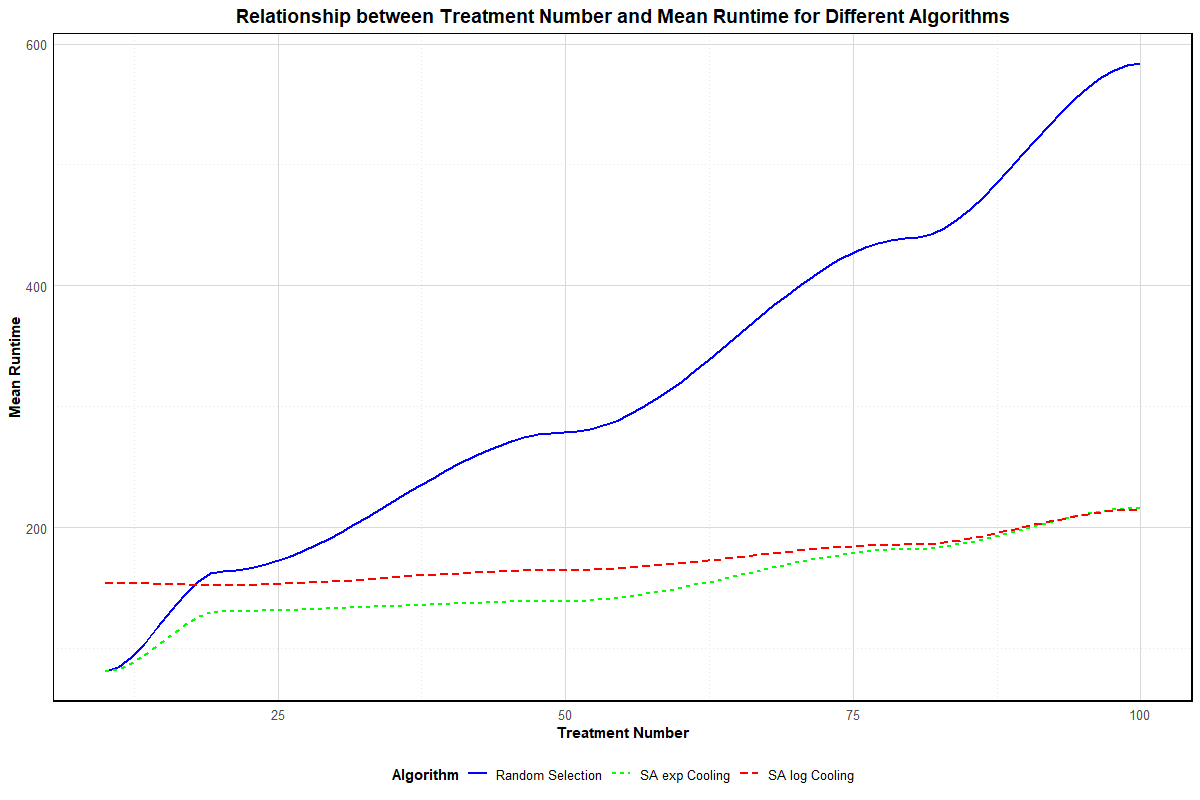
\includegraphics[width=0.7\textwidth,height=\textheight]{images/Rplots/means/trt-vs-t.png}

}

\caption{\#rows v.s. difference)}

\end{figure}%

From the figures, we can see that SA with exponential cooling is the
fastest, while SA with log cooling takes a bit longer, and random
selection requires the longest time. When the number of rows, columns,
and treatments is still small, for the design space is limited and the
randomness of the algorithms, the differences are less noticeable.
However, as these numbers increase, the differences in runtime become
more significant, with random selection showing the fastest increase in
runtime. Overall, the number of rows, columns, and treatments are all
positively correlated with runtime, but the treatment number has a more
direct impact on runtime.

\subsection{Conclusion}\label{conclusion}

Now, we summarize the computational performance of the three algorithms
under constrained computational resources.

First, for random selection, as seen in the analysis above, this
algorithm provides relatively accurate results but requires a longer
runtime. When the number of treatments increases, the runtime
significantly rises. In our simulations, the step-length was set to 3.
Increasing the step-length would allow random selection to search the
design space more extensively but would require more time.

Next is Simulated Annealing (SA). Overall, the iteration speed is faster
compared to random selection. And increasing the number of rows,
columns, and treatments requires more iterations and longer runtime.
Although the log cooling schedule theoretically ensures convergence to
the global optimum, as shown in the simulations above, it may require
more iterations to reach the global optimum. On the other hand, the
exponential cooling schedule converges faster, and it often ends
iteration process early in the simulations. As mentioned earlier, while
it cannot theoretically ensure convergence to the global optimum, it can
provide an approximately optimal solution within a relatively short time
frame under constrained computational resources and avoid local optima
to some extent.

\bookmarksetup{startatroot}

\chapter{Discussion}\label{sec-discuss}

\section{Limitations}\label{limitations}

In this section, we focus on examining the limitations and shortcomings
of our algorithm, along with discussing the practical constraints
observed in the experimental simulation results. Our analysis is
organized into the following parts: computational efficiency and
convergence Rate, balancing multi-objective optimization, and
limitations and generalizability in practical applications.

\subsection{Computational efficiency and convergence
rate}\label{computational-efficiency-and-convergence-rate}

Based on the line plots from the previous section, we observe that the
convergence rate of our three algorithms significantly slow down as they
approach the optimal solution. This often results in giving a
near-optimal solutions, although it performs reasonably well within the
limited number of iterations \(M\) in our simulation. For iterative
methods, the algorithm actually explores the entire design matrix space
by evaluating permutations of the matrix. This causes our algorithms,
especially random selection, to have long runtimes when a large number
of iterations is performed. For certain fixed design assumptions, such
as the diagonal \(\boldsymbol{G}\) matrix and \(\boldsymbol{R}\) matrix
we used previously, an algorithm that optimizes based on matrix
structure could improve efficiency in such cases.

\subsection{Balancing multi-objective
optimization}\label{balancing-multi-objective-optimization}

We aim to optimize A while avoiding bad NB and ED statistics, which
essentially represents a multi-objective optimization problem. In our
current approach, we incorporate filtering steps during random search
permutation generation and SA neighbour generation to ensure that NB and
ED improve gradually throughout the iterations. Although this approach
allows for the stepwise optimization of all three statistics, it fails
to bing in the correlations among them and lacks the ability to balance
and trade off between the three. Using a multi-objective optimization
method would allow us to place these three statistics on an equal
priority level. In our current approach, however, the A-value has
consistently been the primary variable driving changes in the design
matrix.

\subsection{Limitations and generalizability in practical
applications}\label{limitations-and-generalizability-in-practical-applications}

When comparing the computational performance of different algorithms, we
mentioned that such comparisons cannot determine which algorithm is
better. For a deeper exploration of the performance of different
algorithms, a controlled comparison is needed. For example, setting a
common tolerance and allowing all algorithms sufficient time or
iteration count to complete, which would enable a fair comparison of
runtime or iteration numbers. Our analysis of the algorithms is based on
a limited set of constraints, observing and comparing the behaviour of
different algorithms under some conditions.

When discussing model errors, we mentioned using the R matrix for
modelling. For independent plots, using linear models and the R matrix
is very convenient. In \citet{piepho2018neighbor}, the \({AR1}\) model
is suggested as a way to address cases where plots are correlated. We
have not attempted or analysed algorithms using this type of model.

\section{Future Directions}\label{future-directions}

\subsection{Penalty objective
function}\label{penalty-objective-function}

Incorporate a penalty term into the objective function. When adjacent
treatments in the design are the same, this penalty term increases the
value of the objective function, making the optimization process more
likely to avoid having the same treatment in adjacent positions.

For example, we can define a following penalty function. For example we
have a design matrix \(X\), the penalty for self-adjacency is

\[
f(X) = \sum_{(i,j)\in X}I(X_i = X_j)
\] Here \(i\) and \(j\) are different plots next to each other in the
experiment field, and \(I(X_i = X_j)\) is an indicator function equals
to \(1\) if \(i\) plot and \(j\) plot have the same treatment.

So basing on this penalty function, For a certain design \(X\) we change
our function into:

\[
F(X) = \bar{f}_A^{RC} + \lambda \cdot f(X)
\] here \(\lambda < 0\)

Or use A-criteria : \[
G(x) = t\mathcal{A} + (1-t)\cdot f(X)
\] here \(0\leq t \leq 1\) and we minimize it

Usually we have such mathematical programming of inequality constrained
optimization problem: we minimize objective function \(f_0(x)\) with
inequality constrains \(f_i(x)\leq 0, i\in I=\{1,2,\cdots,m\}\).And we
have a well-known penalty function for this problem is \[
F (x, \rho) = f_0(x) + \rho \sum_{i\in I}max\{f_i(x),0\}
\] and a corresponding constrained penalty optimization problem is to
minimize penalty function \(F_2 (x, \rho)\), detailed information in
\citet{meng2013exactness}

\subsection{Algorithm improvment}\label{algorithm-improvment}

\subsubsection{SA-based multiobjective optimization
algorithms}\label{sa-based-multiobjective-optimization-algorithms}

When discussing the A-value, NB statistic, and ED statistic, our goal is
actually to find a process that can simultaneously optimize all three,
or finding a balance between three statistic criteria.SA is often used
in combinatorial optimization problems, as we are using it here to
optimize the arrangement of treatment plots. \citet{suman2006survey}
claim that in recent studies, SA has been applied in many
multi-objective optimization problems, because of its simplicity and
capability of producing a Pareto set of solutions in single run with
very little computational cost.

We say a solution is non-dominated if none of its objective values can
be improved without worsening at least one other objective. The Pareto
set (or Pareto front) is a set of non-dominated solutions in a
multi-objective optimization problem. \citet{suman2006survey} introduce
several SA for multi-objective optimization.

SA-based multi-objective optimization algorithms given by
\citet{suppapitnarm2000simulated} is a promising approach. Instead of
Equation~\ref{eq-prob} and using permutation filtering, they give
probability step write as this form \[
P = \min(1, \Pi_{i=1}^N\exp\{\frac{-\bigtriangleup s_i}{T_i}\})
\] Here \(N\) is the number of objective functions, and for each
objective function \(i\), \(\bigtriangleup s_i\) is the difference of
objective function between two solution and \(T_i\) is the current
temperature. Control the optimization rates of different objective
functions by setting different cooling schedules for each.

\subsubsection{Memory-Based Optimization Algorithms - TABU
search}\label{memory-based-optimization-algorithms---tabu-search}

Same with SA, Tabu Search is an optimization algorithm used for solving
combinatorial problems. It is a type of local search method that
enhances basic hill-climbing algorithms by using memory structures to
avoid revisiting previously explored solutions, introduced in
\citet{butler2013model}. This helps the search process escape from local
optima and encourages exploration of new areas in the solution space.
Tabu Search maintains a tabu list, a short-term memory that keeps track
of recent moves or solutions that should not be revisited for a certain
number of iterations. This is mathematically represented as a set
\(\mathcal{T}\) where recent solutions \(X_t\) are stored for a fixed
period \(k\) iterations: \[
\mathcal{T} = \{x_t|t \in [t-k,t)\}
\] If a solution \(x' \in \mathcal{T}\), \(x'\) is considered ``tabu''
and cannot be revisited. Therefore, besides our two approaches
here---random search with step-length and SA that probabilistically
accepts worse objective function values---this type of short-term
memory-enhanced algorithm (Memory-Enhanced Algorithms) helps ensure
efficient computation, minimizing resource consumption while maximizing
exploration within the solution space and helping escape local optima.

\bookmarksetup{startatroot}

\chapter*{References}\label{references}
\addcontentsline{toc}{chapter}{References}

\markboth{References}{References}

\renewcommand{\bibsection}{}
\bibliography{ref.bib}

\cleardoublepage
\phantomsection
\addcontentsline{toc}{part}{Appendices}
\appendix

\chapter{Tools}\label{sec-tools}

This thesis was written using \href{https://quarto.org/}{Quarto 1.5.31}
\citep{quarto} and the following system and R packages:

\begin{verbatim}
- Session info ---------------------------------------------------------------
 setting  value
 version  R version 4.3.1 (2023-06-16)
 os       macOS 15.0.1
 system   aarch64, darwin20
 ui       X11
 language (EN)
 collate  en_US.UTF-8
 ctype    en_US.UTF-8
 tz       Australia/Sydney
 date     2024-10-20
 pandoc   3.1.11 @ /Applications/RStudio.app/Contents/Resources/app/quarto/bin/tools/aarch64/ (via rmarkdown)

- Packages -------------------------------------------------------------------
 package     * version date (UTC) lib source
 cli           3.6.3   2024-06-21 [1] CRAN (R 4.3.3)
 digest        0.6.35  2024-03-11 [1] CRAN (R 4.3.1)
 evaluate      1.0.0   2024-09-17 [1] CRAN (R 4.3.3)
 fastmap       1.1.1   2023-02-24 [1] CRAN (R 4.3.0)
 here          1.0.1   2020-12-13 [1] CRAN (R 4.3.0)
 htmltools     0.5.8   2024-03-25 [1] CRAN (R 4.3.1)
 jsonlite      1.8.8   2023-12-04 [1] CRAN (R 4.3.1)
 knitr         1.48    2024-07-07 [1] CRAN (R 4.3.3)
 later         1.3.2   2023-12-06 [1] CRAN (R 4.3.1)
 processx      3.8.4   2024-03-16 [1] CRAN (R 4.3.1)
 ps            1.7.6   2024-01-18 [1] CRAN (R 4.3.1)
 quarto        1.4     2024-03-06 [1] CRAN (R 4.3.1)
 Rcpp          1.0.12  2024-01-09 [1] CRAN (R 4.3.1)
 rlang         1.1.4   2024-06-04 [1] CRAN (R 4.3.3)
 rmarkdown     2.26    2024-03-05 [1] CRAN (R 4.3.1)
 rprojroot     2.0.4   2023-11-05 [1] CRAN (R 4.3.1)
 rstudioapi    0.16.0  2024-03-24 [1] CRAN (R 4.3.1)
 sessioninfo   1.2.2   2021-12-06 [1] CRAN (R 4.3.0)
 xfun          0.47    2024-08-17 [1] CRAN (R 4.3.3)
 yaml          2.3.10  2024-07-26 [1] CRAN (R 4.3.3)

 [1] /Library/Frameworks/R.framework/Versions/4.3-arm64/Resources/library

------------------------------------------------------------------------------
\end{verbatim}


\backmatter


\end{document}
